% Format teze zasnovan je na paketu memoir
% http://tug.ctan.org/macros/latex/contrib/memoir/memman.pdf ili
% http://texdoc.net/texmf-dist/doc/latex/memoir/memman.pdf
% 
% Prilikom zadavanja klase memoir, navedenim opcijama se podešava 
% veličina slova (12pt) i jednostrano štampanje (oneside).
% Ove parametre možete menjati samo ako pravite nezvanične verzije
% mastera za privatnu upotrebu (na primer, u b5 varijanti ima smisla 
% smanjiti 
\documentclass[12pt,oneside]{memoir} 

% Paket koji definiše sve specifičnosti master rada Matematičkog fakulteta
\usepackage[latinica]{matfmaster} 
%
% Podrazumevano pismo je ćirilica.
%   Ako koristite pdflatex, a ne xetex, sav latinički tekst na srpskom jeziku
%   treba biti okružen sa \lat{...} ili \begin{latinica}...\end{latinica}.
%
% Opcija [latinica]:
%   ako želite da pišete latiniciom, dodajte opciju "latinica" tj.
%   prethodni paket uključite pomoću: \usepackage[latinica]{matfmaster}.
%   Ako koristite pdflatex, a ne xetex, sav ćirilički tekst treba biti
%   okružen sa \cir{...} ili \begin{cirilica}...\end{cirilica}.
%
% Opcija [biblatex]:
%   ako želite da koristite reference na više jezika i umesto paketa
%   bibtex da koristite BibLaTeX/Biber, dodajte opciju "biblatex" tj.
%   prethodni paket uključite pomoću: \usepackage[biblatex]{matfmaster}
%
% Opcija [b5paper]:
%   ako želite da napravite verziju teze u manjem (b5) formatu, navedite
%   opciju "b5paper", tj. prethodni paket uključite pomoću: 
%   \usepackage[b5paper]{matfmaster}. Tada ima smisla razmisliti o promeni
%   veličine slova (izmenom opcije 12pt na 11pt u \documentclass{memoir}).
%
% Naravno, opcije je moguće kombinovati.
% Npr. \usepackage[b5paper,biblatex]{matfmaster}

% Pomoćni paket koji generiše nasumičan tekst u kojem se javljaju sva slova
% azbuke (nema potrebe koristiti ovo u pravim disertacijama)
\usepackage[latinica]{pangrami}

% Datoteka sa potrebnim paketima
\usepackage{listings}
\usepackage{textcomp}
\usepackage{xcolor}

% \setmonofont{Consolas}
\definecolor{bluekeywords}{rgb}{0,0,1}
\definecolor{greencomments}{rgb}{0,0.5,0}
\definecolor{redstrings}{rgb}{0.64,0.08,0.08}
\definecolor{xmlcomments}{rgb}{0.5,0.5,0.5}
\definecolor{types}{rgb}{0.17,0.57,0.68}

\usepackage{amsmath}

\usepackage[figure]{algorithm}
\floatname{algorithm}{Pseudokod}
\usepackage[noend]{algpseudocode}

\usepackage{listings}
\lstset{
    language=csh,
    captionpos=b,
    % aboveskip=5pt,
    % belowskip=5pt,
    numbers=left, 
    numberstyle=\tiny,
    frame=single,
    framesep=10pt,
    showspaces=false,
    showtabs=false,
    breaklines=true,
    showstringspaces=false,
    breakatwhitespace=true,
    escapeinside={(*@}{@*)},
    commentstyle=\color{greencomments},
    morekeywords={partial, var, value, get, set},
    keywordstyle=\color{bluekeywords},
    stringstyle=\color{redstrings},
    basicstyle=\ttfamily\footnotesize,
    tabsize=4,
    framexleftmargin=1.5em,
    xleftmargin=2em,
    % escapechar=\&,
    classoffset=1, 
    morekeywords={ until, final, abstract, event, new, struct,
    as, explicit, null, switch,
    base, extern, object, this,
    bool, false, operator, throw,
    break, finally, out, true,
    byte, fixed, override, try,
    case, float, params, typeof,
    catch, for, private, uint,
    char, foreach, protected, ulong,
    checked, goto, public, unchecked,
    class, if, readonly, unsafe,
    const, implicit, ref, ushort,
    continue, in, return, using,
    decimal, int, sbyte, virtual,
    default, interface, sealed, volatile,
    delegate, internal, short, void,
    do, is, sizeof, while,
    double, lock, stackalloc,
    else, long, static,
    enum, namespace, string, 
    >,<,.,;,,,-,!,=,~},
    classoffset=0,
}

% \lstset {
%     frame=single,
%     framesep=10pt,
%     xrightmargin=-25pt,
%     showstringspaces=false,
%     upquote=true,
%     commentstyle=\color{commentgreen},
%     keywordstyle=\color{blue},
%     stringstyle=\color{red},
%     basicstyle=\footnotesize\ttfamily,
%     emphstyle={\color{blue}},
%     escapechar=\&,
%     % keyword highlighting
%     classoffset=1, % starting new class
%     morekeywords={ abstract, event, new, struct,
%     as, explicit, null, switch,
%     base, extern, object, this,
%     bool, false, operator, throw,
%     break, finally, out, true,
%     byte, fixed, override, try,
%     case, float, params, typeof,
%     catch, for, private, uint,
%     char, foreach, protected, ulong,
%     checked, goto, public, unchecked,
%     class, if, readonly, unsafe,
%     const, implicit, ref, ushort,
%     continue, in, return, using,
%     decimal, int, sbyte, virtual,
%     default, interface, sealed, volatile,
%     delegate, internal, short, void,
%     do, is, sizeof, while,
%     double, lock, stackalloc,
%     else, long, static,
%     enum, namespace, string, 
%     >,<,.,;,,,-,!,=,~},
%     keywordstyle=\color{blue},
%     classoffset=0,
% }

% Datoteka sa literaturom u BibTex tj. BibLaTeX/Biber formatu
\bib{references}

% Ime kandidata na srpskom jeziku (u odabranom pismu)
\autor{Ivan Ristović}
% Naslov teze na srpskom jeziku (u odabranom pismu)
\naslov{Jezički invarijantna provera semantičke ekvivalentnosti strukturno sličnih segmenata imperativnog koda}
% Godina u kojoj je teza predana komisiji
\godina{2020}
% Ime i afilijacija mentora (u odabranom pismu)
\mentor{doc. dr Milena \textsc{Vujošević-Janičić}\\ Univerzitet u Beogradu, Matematički fakultet}
% Ime i afilijacija prvog člana komisije (u odabranom pismu)
\komisijaA{prof. dr Filip \textsc{Marić}\\ Univerzitet u Beogradu, Matematički fakultet}
% Ime i afilijacija drugog člana komisije (u odabranom pismu)
\komisijaB{doc. dr Milan \textsc{Banković}\\ Univerzitet u Beogradu, Matematički fakultet}
% Ime i afilijacija trećeg člana komisije (opciono)
% \komisijaC{}
% Ime i afilijacija četvrtog člana komisije (opciono)
% \komisijaD{}
% Datum odbrane (odkomentarisati narednu liniju i upisati datum odbrane ako je poznat)
% \datumodbrane{}

% Apstrakt na srpskom jeziku (u odabranom pismu)
\apstr{%
Apstraktno sintaksičko stablo (engl. abstract syntax tree, skraćeno AST) nastaje kao rezultat parsiranja ulaznog programa i predstavlja osnovu za semantičku analizu koda. U okviru semantičke analize koda veoma su važne analize koje omogućavaju obezbeđivanje visokog kvaliteta softvera, bilo kroz analize koje uključuju statičko otkrivanje grešaka u kodu ili kroz analize koje imaju za cilj automatsku transformaciju koda u semantički ekvivalentan oblik sa nekom željenom karakteristikom (na primer, u okviru procesa refaktorisanja koda). Međutim, apstraktno sintaksičko stablo je specifično za konkretan viši programski jezik i na osnovu njega se ne mogu porediti karakteristike programa napisanih u različitim programskim jezicima, što je posebno važno u okviru procesa migracije na nove tehnologije. Ovaj rad opisuje opštu AST reprezentaciju za imperativne programske jezike sa ciljem njene primene u analizi semantičke ekvivalentnosti implementacija algoritama u različitim programskim jezicima. Koncept opšteg AST i semantičkih upoređivača je pružen kroz aplikaciju LICC, implementiranu u programskom jeziku C\# koristeći ANTLR4 generator parsera. LICC dozvoljava kreiranje apstrakcije na osnovu zadate gramatike imperativnog programskog jezika, pri čemu je koncept prikazan na primeru jednostavnog pseudokoda, kao i na programskim jezicima C i Lua.
}

% Ključne reči na srpskom jeziku (u odabranom pismu)
\kljucnereci{Apstraktno sintaksičko stablo, AST, ANTLR, opšta AST apstrakcija, semantička ekvivalentnost imperativnih segmenata koda}

\begin{document}
% ==============================================================================
% Uvodni deo teze
\frontmatter
% ==============================================================================
% Naslovna strana
\naslovna
% Strana sa podacima o mentoru i članovima komisije
\komisija
% Strana sa posvetom (u odabranom pismu)
\posveta{Zahvaljujem se mentoru doc.~Mileni Vujošević-Janičić na inspiraciji, pomoći i savetima.}
% Strana sa podacima o disertaciji na srpskom jeziku
\apstrakt
% Sadržaj teze
\tableofcontents*

% ==============================================================================
% Glavni deo teze
\mainmatter
% ==============================================================================

\chapter{Uvod}
\label{chp:Intro}

Apstraktno sintaksičko stablo (engl. \emph{abstract syntax tree}, skr. \emph{AST}) programa ima značajnu ulogu u procesu kreiranja izvršivog programa od izvornog koda. AST nastaje parsiranjem izvornog koda, kao rezultat apstrahovanja stabla parsiranja koje generiše \emph{parser}. Parser čita izvorni k\^od i pokušava da u njemu pronađe primene određenih pravila jezika čiji je k\^od dizajniran da parsira. Svaki programski jezik ima specifična sintaksna pravila pa su stoga i skupovi pravila (tzv. \emph{gramatike}) programskih jezika raznorodni, što se zatim prenosi i na generisana stabla parsiranja. Stablo parsiranja se apstrahuje tako što se iz njega izvuku samo bitne sintaksne a uklone neke tehničke informacije.

Ovakva apstrakcija se najpre koristi u semantičkoj analizi programa koju vrši prevodilac nakon faze parsiranja i provere sintaksne ispravnosti koda. Ukoliko program prođe semantičke provere, prelazi se na prevođenje istog u međureprezentaciju i fazu optimizacije. Nakon faze optimizacije sledi generisanje asemblerskog koda koji se zatim prevodi u mašinski k\^od.

AST, zbog svoje uloge u semantičkoj analizi, može poslužiti i za analizu programa pre samog prevođenja, kroz proces poznat pod nazivom \emph{statička analiza}. Posmatranje programa kroz AST pruža mogućnost za poređenje dva programa na apstraktnom nivou. Jedna primena ove ideje u okviru statičke analize može biti provera semantičke ekvivalentnosti. Provera semantičke ekvivalentnosti dva programa je neodlučiv problem u opštem slučaju, međutim pod određenim pretpostavkama koje pojednostavljuju problem moguće je dizajnirati algoritme koji daju smislene rezultate u praksi. Jedna od često korišćenih pretpostavki je pretpostavka sličnosti strukture dva programa. Interesantno, provera da li dva programa zadovoljavaju ovu premisu se može proveriti posmatranjem izgleda i sličnosti u strukturi na apstraktnom nivou --- problem koji se može rešiti primenom algoritama za rad sa stablima jer je u pitanju AST (ali i grafovima uopšte, jer je stablo specijalizacija grafa).

Iako veoma konceptualno moćan alat, AST je ipak specifičan za konkretni programski jezik s obzirom da nastaje od stabla parsiranja koje je usko vezano za gramatiku konkretnog programskog jezika. Motivacija za ovaj rad dolazi od nepostojanja opštih apstrakcija sintaksičkih stabala koje bi se mogle koristiti za analizu programa napisanih u različitim programskim jezicima. Iako je broj programskih jezika danas veoma veliki, u okviru iste programske paradigme jezici moraju implementirati koncepte koji su potrebni da bi se programiralo u toj paradigmi i ta zajednička svojstva se mogu iskoristiti za formiranje zajedničke apstrakcije. 

U ovom radu će biti predstavljena opšta AST apstrakcija za imperativne programske jezike, sa ciljem da se omogući zajednička apstraktna reprezentacija velikog broja imperativnih jezika, pa čak i onih koji pripadaju skript paradigmi. Njena upotreba će biti demonstrirana na problemu semantičke ekvivalentnosti dobijenih apstrakcija kroz naivni algoritam poređenja simboličkih promenljivih. Štaviše, na apstraktnom nivou nije važno od kog se programskog jezika dobio AST, što može imati primenu u procesu migracije na nove tehnologije.

Naravno, semantička ekvivalentnost se ne mora zasnivati na apstrahovanju programa, već se takođe često rešava spuštanjem na nivo međukoda između višeg programskog jezika i asemblera. U nekim slučajevima se može iči i do asemblera pa i mašinskog jezika. Ukoliko bi se posmatrali asemblerski ili mašinski kod, vršilo bi se poređenje kodova prilagođenih određenoj arhitekturi procesora. U ovom radu je odabran AST-zasnovan pristup, s obzirom na važnosti i značaj apstraktnih sintaksičkih stabala, ali i zbog nedostatka opštih apstrakcija.

U poglavlju \ref{chp:RelevantTerms} će biti opisani relevantni pojmovi potrebni za razumevanje rada uz akcenat na apstraktnim sintaksičkim stablima i procesu njihovog dobijanja. Opšta AST apstrakcija za imperativne jezike biće opisana u poglavlju \ref{chp:MyAST}, a njena upotreba u problemu odlučivanja semantičke ekvivalentnosti kao i sam algoritam za poređenje opštih apstrakcija biće opisani u poglavlju \ref{chp:ASTComparing}. Implementacija apstrakcije i algoritma semantičkog poređenja će biti opisana u poglavlju \ref{chp:Implementation}. Na kraju, biće dati glavni zaključci ovog rada kao i moguća unapređenja i budući koraci. 

\chapter{AST - generisanje i korišćenje}
\label{chp:RelevantTerms}

U ovom poglavlju će biti opisani koncepti i alati čije je razumevanje potrebno kako bi se razumeo opis dalje apstrakcije i implementacije samog programa. Umesto analize samog sadržaja izvornog koda analizira se \emph{apstraktno sintaksičko stablo}, opisano u odeljku \ref{sec:AST}. Kako bi se od izvornog koda došlo do stabla parsiranja a potom i do apstraktnog sintaksičkog stabla, koriste se \emph{lekseri} i \emph{parseri}. S obzirom da je cilj kreirati univerzalnu reprezentaciju, biće neophodno kreirati leksere i parsere za proizvoljne gramatike. Više reči o samom procesu dobijanja stabla parsiranja od izvornog koda i alatima koji mogu da generišu leksere i parsere biće u odeljku \ref{sec:ParsingGrammars}, sa akcentom na alat \emph{Another Tool For Language Recognition} \cite{ANTLR}, u daljem tekstu \emph{ANTLR}. Da bi se dobijena stabla koristila, neophodno je poznavati \emph{obrasce za projektovanje} opisane u odeljku \ref{sec:DesignPatterns} koji pružaju gotova rešenja za česte probleme koji se u ovom radu koriste za pružanje interfejsa obilaska stabala i izračunavanja vrednosti nad istim.

\section{Apstraktna sintaksička stabla}
\label{sec:AST}

Kako bi se k\^od pisan u nekom programskom jeziku (\emph{izvorni fajl}) preveo u k\^od koji će se izvršavati na nekoj mašini (\emph{izvršivi fajl}), prevodilac izvršava određene korake. Prvi korak je prepoznavanje gradivnih elemenata programskog jezika koji se nazivaju \emph{lekseme}, nalik na prepoznavanje reči u rečenicama govornog jezika, i raspodela leksema u grupe po funkciji (nalik na funkcije reči u govornom jeziku --- subjekti, predikati, objekti itd.). Nakon prepozavanja leksema, proverava se da li niz prepoznatih leksema ispunjava pravila odnosno \emph{sintaksu} programskog jezika, nalik na proveru da li se složene govorne rečenice sastoje od subjekta i predikta u određenom redosledu. Na kraju se proverava značenje odnosno \emph{semantika} koda, nalik na proveru da li govorne rečenice, iako sintaksno pravilne, imaju smisla. Deo prevodioca koji određuje da li je izvorni k\^od ispravno formiran u terminima leksike, sintakse i semantike se naziva \emph{prednji deo} (engl. \emph{front end}). Ukoliko je izvorni k\^od ispravan, prednji deo kreira \emph{međureprezentaciju} koda (engl. \emph{intermediate representation}, u daljem tekstu \emph{IR}) nad kojom se vrše optimizacije koda i koja se koristi za dalji proces prevođenja. Ukoliko to nije slučaj, prevođenje ne uspeva i programeru se daje poruka sa obrazloženjem zašto prevođenje nije uspelo \cite{EngineeringCompilers}.

Za potrebe ovog rada, što se procesa prevođenja tiče, dovoljno je poznavanje pomenutih procesa koje izvodi prednji deo, stoga neće biti reči o ostalim koracima u fazi prevođenja (optimizovanje, generisanje IR). Zainteresovani čitalac može više detalja pronaći u \cite{DragonBook}, \cite{EngineeringCompilers} i \cite{CompilerConstruction}. 

Pretpostavimo da želimo da prevedemo izvorni k\^od pisan u programskom jeziku C sa slike \ref{fig:CompilationProcessInit}. Primetimo da postoji greška u datom kodu --- simbol \texttt{c} koji se koristi u dodeli u liniji $7$ će biti prepoznat kao identifikator koji ne odgovara nijednoj deklarisanoj promenljivoj --- stoga ne možemo prevesti ovaj k\^od. Ovo nije greška u sintaksi --- izraz \texttt{a+c} je validan u programskom jeziku C. Problem će postati vidljiv tek nakon parsiranja izvornog koda i provere ispunjenosti sintaksih pravila, tačnije u fazi semantičke provere. Stoga se ovakve greške nazivaju \emph{semantičke greške}, dok se greške u sintaksi nazivaju \emph{sintaksne greške}.

\begin{figure}[h!]
\begin{lstlisting}
#include<stdio.h>
#define T int

int main()
{
    T a, b;
    a = a + c;        // c nije deklarisano
    printf("%d", a);
    return 0;
}
\end{lstlisting}
\caption{Primer izvornog koda sa semantičkom greškom (C).}
\label{fig:CompilationProcessInit}
\end{figure}

Pre nego što prednji kraj prevodioca dobije k\^od koji treba da prevede u međureprezentaciju, vrši se \emph{pretprocesiranje} od strane programa koji se naziva \emph{pretprocesor}. U fazi pretprocesiranja se izvode samo tekstualne operacije kao što su brisanje komentara ili zamena makroa u jezicima kao što je C. Rezultat rada pretprocesora za izvorni k\^od sa slike \ref{fig:CompilationProcessInit} se može videti na slici \ref{fig:CompilationProcessPrep}\footnote{U nekim implementacijama C standardne biblioteke, moguće je da se poziv funckije \texttt{printf} zameni pozivom funkcije \texttt{fprintf} sa ispisom na \texttt{stdout}. U standardu se propisuje da funkcije kao što je \texttt{printf} mogu biti implementirane kao makroi. Izlaz na slici \ref{fig:CompilationProcessPrep} je generisan od strane \texttt{GCC 7.4.0} po C11 standardu i ovo nije slučaj u datom okruženju.}.

\begin{figure}[h!]
\begin{lstlisting}
# 1 "<stdin>"
# 1 "<built-in>"
# 1 "<command-line>"
# 31 "<command-line>"
# 1 "/usr/include/stdc-predef.h" 1 3 4

...

extern char *ctermid (char *__s) __attribute__ ((__nothrow__ , __leaf__));
# 840 "/usr/include/stdio.h" 3 4
extern void flockfile (FILE *__stream) __attribute__ ((__nothrow__ , __leaf__));
extern int ftrylockfile (FILE *__stream) __attribute__ ((__nothrow__ , __leaf__)) ;
extern void funlockfile (FILE *__stream) __attribute__ ((__nothrow__ , __leaf__));
# 868 "/usr/include/stdio.h" 3 4
# 2 "<stdin>" 2
# 2 "<stdin>"

int main()
{
    int a, b;
    a = a + c;
    printf("%d", a);
    return 0;
}
\end{lstlisting}
\caption{Prikaz rezultata rada pretprocesora za izvorni k\^od sa slike \ref{fig:CompilationProcessInit}. Pritom, prikazano je samo par linija sa početka i kraja izlaza pretprocesora --- k\^od iznad \texttt{main} funkcije je uključen iz \texttt{stdio.h} zaglavlja.}
\label{fig:CompilationProcessPrep}
\end{figure}

U toku faze leksičke analize, kako prevodilac ne bi radio nad sirovim karakterima izvornog koda, potrebno je izvršiti transformaciju karaktera izvornog koda. Prevodilac ima u vidu elemente programskog jezika i šablone za njihovo prepoznavanje. Lekseme su one sekvence karaktera izvornog koda koje zadovoljavaju ove šablone. Lekseme se dalje razvrstavaju u kategorije, tzv. \emph{tokene} --- ključne reči, operatore, promenljive itd. Proces dobijanja tokena od izvornog koda se naziva \emph{tokenizacija}. Komponenta prednjeg dela koja vrši tokenizaciju se naziva \emph{skener} ili \emph{lekser}. Pojednostavljen primer šablona koje lekser pokušava da prepozna se mogu videti na slici \ref{fig:CLexerExample}. Primer izlaza leksera za izlaz pretprocesora sa slike \ref{fig:CompilationProcessPrep} se može videti na slici \ref{fig:CompilationProcessLex}.

\begin{figure}[h!]
\begin{lstlisting}[language={}]
Identifier 
    : IdentifierNondigit (IdentifierNondigit | Digit)*
    ;
IdentifierNondigit  
    : Nondigit
    | UniversalCharacterName
    ;
Nondigit 
    : [a-zA-Z_]
    ;
Digit 
    : [0-9]
    ;
\end{lstlisting}
\caption{Primer delimične definicije tokena za ime promenljive po C11 standardu.}
\label{fig:CLexerExample}
\end{figure}

\begin{figure}[h!]
\begin{lstlisting}[language={}]
identifier 'main'	 [LeadingSpace]	Loc=<sample.c:3:5>
l_paren '('		Loc=<sample.c:3:9>
r_paren ')'		Loc=<sample.c:3:10>
l_brace '{'	 [StartOfLine]	Loc=<sample.c:4:1>
int 'int'	 [StartOfLine] [LeadingSpace]	Loc=<sample.c:5:5>
identifier 'a'	 [LeadingSpace]	Loc=<sample.c:5:9>
comma ','		Loc=<sample.c:5:10>
identifier 'b'	 [LeadingSpace]	Loc=<sample.c:5:12>
semi ';'		Loc=<sample.c:5:13>
identifier 'a'	 [StartOfLine] [LeadingSpace]	Loc=<sample.c:6:5>
equal '='	 [LeadingSpace]	Loc=<sample.c:6:7>
identifier 'a'	 [LeadingSpace]	Loc=<sample.c:6:9>
plus '+'	 [LeadingSpace]	Loc=<sample.c:6:11>
identifier 'c'	 [LeadingSpace]	Loc=<sample.c:6:13>
semi ';'		Loc=<sample.c:6:14>
identifier 'printf'	 [StartOfLine] [LeadingSpace]	Loc=<sample.c:7:5>
l_paren '('		Loc=<sample.c:7:11>
string_literal '"%d"'		Loc=<sample.c:7:12>
comma ','		Loc=<sample.c:7:16>
identifier 'a'	 [LeadingSpace]	Loc=<sample.c:7:18>
r_paren ')'		Loc=<sample.c:7:19>
semi ';'		Loc=<sample.c:7:20>
return 'return'	 [StartOfLine] [LeadingSpace]	Loc=<sample.c:8:5>
numeric_constant '0'	 [LeadingSpace]	Loc=<sample.c:8:12>
semi ';'		Loc=<sample.c:8:13>
r_brace '}'	 [StartOfLine]	Loc=<sample.c:9:1>
eof ''		Loc=<sample.c:9:2>
\end{lstlisting}
\caption{Proces tokenizacije koda sa slike \ref{fig:CompilationProcessPrep} (generisano pomoću kompajlera \texttt{clang} \cite{Clang}).}
\label{fig:CompilationProcessLex}
\end{figure}

Nakon faze skeniranja potrebno je proveriti da li niz pročitanih tokena zadovoljava sintaksu programskog jezika. Pevodilac stoga mora da uporedi strukturu koda sa unapred definisanom strukturom za određeni programski jezik što zahteva formalnu definiciju sintakse jezika. Programski jezik možemo posmatrati kao skup \emph{pravila} pod imenom \emph{gramatika} \cite{ContextFreeGrammars}. Na slici \ref{fig:CompilationProcessGram} se može videti deo gramatike programskog jezika C. Proces provere zadovoljenosti sintaksnih pravila se naziva \emph{parsiranje}, a komponenta prednjeg dela koja vrši parsiranje se naziva \emph{parser}.\footnote{Moderni kompajleri često nemaju odvojene faze skeniranja i parsiranja, već se skeniranje odvija paralelno sa fazom parsiranja. Međutim, to nas ne sprečava da ispišemo tokene onda kada se oni prepoznaju, što to je demonstrirano na slici \ref{fig:CompilationProcessLex}.}

\begin{figure}[h!]
\begin{lstlisting}[language={}]
declarationList
    :   declaration
    |   declarationList declaration
    ;
declaration
    :   declarationSpecifiers initDeclaratorList ';'
    | 	declarationSpecifiers ';'
    |   staticAssertDeclaration
    ;
\end{lstlisting}
\caption{Prikaz para pravila iz gramatike programskog jezika C po standardu C11.}
\label{fig:CompilationProcessGram}
\end{figure}

Parser, imajući u vidu gramatiku jezika, kreira \emph{stablo parsiranja} (eng. \emph{parse tree} ili \emph{derivation tree}). Takvo stablo i dalje sadrži sve relevantne informacije o izvornom kodu. Vizuelni prikaz rada parsera za gramatiku sa slike C11 i izvornog koda sa slike \ref{fig:CompilationProcessInit} je dat na slici \ref{fig:CompilationProcessPars}. Stablo parsiranja se koristi u narednim fazama prevođenja.

\begin{figure}[h!]
\centering
\scalebox{0.95}[1.3] {
    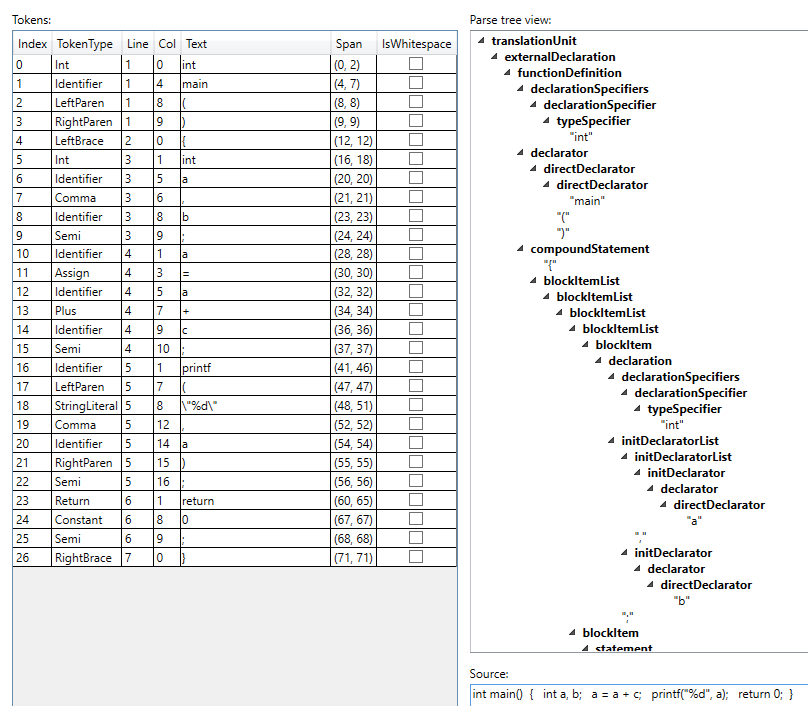
\includegraphics[width=\textwidth]{images/parse_tree.png}
}
\caption{Prikaz dela stabla parsiranja koje generiše parser kreiran od strane alata ANTLR4 \cite{ANTLR} za k\^od sa slike \ref{fig:CompilationProcessPrep}.}
\label{fig:CompilationProcessPars}
\end{figure}

Stablo parsiranja sadrži sve informacije potrebne u fazi parsiranja uključujući detalje korisne samo za parser prilikom provere ispunjenosti gramatičkih pravila. Sa druge strane, \emph{apstraktno sintaksičko stablo} sadrži samo sintaksičku strukturu u jednostavnijoj formi. Na slici \ref{fig:CompilationProcessPars1} se može videti koliko stablo parsiranja može biti kompleksno čak i za jednostavne aritmetičke izraze. Razlog kompleksnosti u ovom slučaju dolazi iz rekurzivnih pravila iz C11 gramatike. Parseru su sve ove informacije neophodne ali za naredne analize i proces prevođenja one nisu potrebne i zato se stablo parsiranja apstrahuje. Na primer, jedina važna semantička odlika izraza \texttt{a+c} je da je to zbir vrednosti nekih promenljivih. Na slici \ref{fig:ASTVariants} se mogu videti različita apstraktna sintaksička stabla za pomenuti izraz, ali takođe i za malo složenije izraze. Podrazumeva se, naravno, da je ulaz već tokenizovan. 

\begin{figure}[h!]
\centering
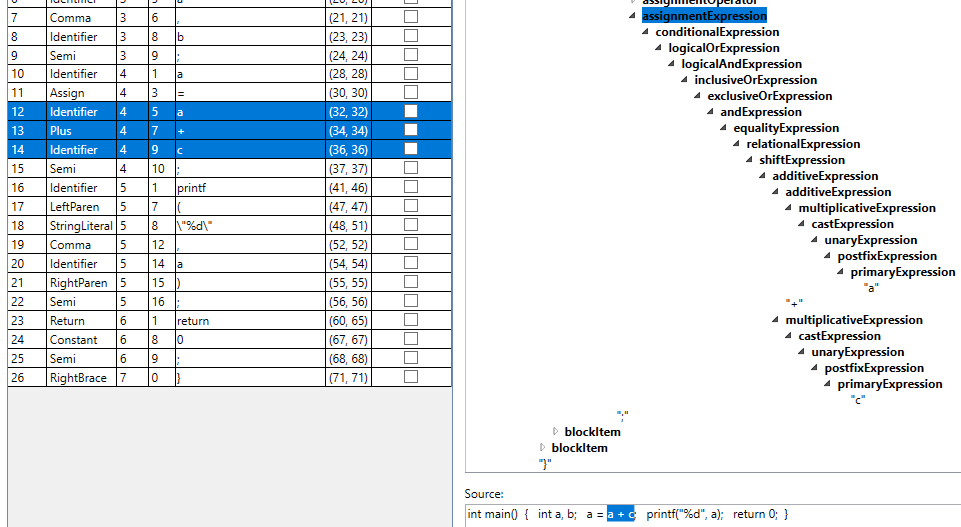
\includegraphics[scale=0.55]{images/parse_tree_expr.png}
\caption{Prikaz kompleksnosti stabla parsiranja za izraz 
\texttt{a+c} u C11 gramatici.} 
\label{fig:CompilationProcessPars1}
\end{figure}

\begin{figure}[h!]
\centering
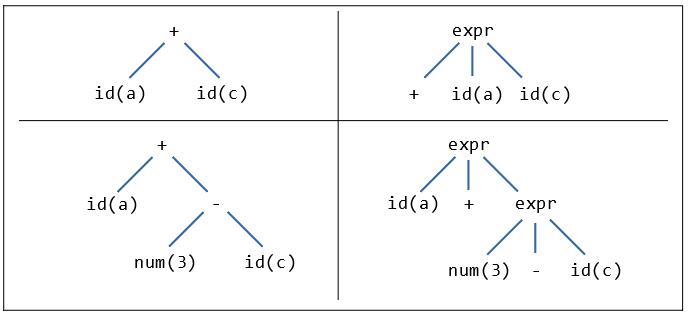
\includegraphics[scale=0.7]{images/ast.png}
\caption{AST varijante bez regularnosti (levo) i sa regularnošću (desno) za izraze \texttt{a+c} (gore) i \texttt{a+(3-c)} (dole).} 
\label{fig:ASTVariants}
\end{figure}

Uloga apstraktnog sintaksičkog stabla \cite{FormalSyntaxAndSemantics} je da pokaže semantiku strukture koda preko stabla. Kao što se vidi na slici \ref{fig:ASTVariants}, postoji određeni nivo slobode prilikom njihovog kreiranja. Generalno, \emph{terminalni simboli} --- simboli koji predstavljaju listove stabla parsera --- koji odgovaraju operatorima i naredbama se podižu naviše i postaju koreni podstabala, dok se njihovi operandi ostavljaju kao njihovi potomci u stablu. Desna stabla sa slike ne prate u potpunosti ovaj princip, ali se takođe koriste zbog regularnosti izraza --- ukoliko binarni izraz posmatramo kao apstrakciju, za implementaciju je lakše koristiti ovakav tip apstraktnih sintaksičkih stabala i stoga će biti korišćen kasnije u implementaciji opšte apstrakcije. Primetimo takođe da se u stablima za izraz \texttt{a+(3-c)} (dole) implicitno sačuvala informacija o prioritetu operacije oduzimanja u izrazu. Jasno je, dakle, da se računanje vrednosti aritmetičkih izraza onda vrši kretanjem od listova stabla ka korenu. Takođe, pošto je apstraktno sintaksičko stablo apstrakcija stabla parsiranja, više semantički ekvivalentnih izraza može imati isto apstraktno sintaksičko stablo ali različito stablo parsiranja; na primer, ako razmatramo izraz \texttt{(a+5)-x/2} i izraz \texttt{a+5-(x/2)}.


\section{Parsiranje gramatika programskih jezika}
\label{sec:ParsingGrammars}

Ukoliko imamo gramatiku proizvoljnog programskog jezika, postavlja se pitanje: 
\begin{quote}
    Da li je moguće definisati postupak i zatim napraviti program koji će generisati kodove leksera i parsera napisane u nekom specifičnom programskom jeziku za proizvoljnu gramatiku datu na ulazu?
\end{quote}
Odgovor je potvrdan i postoji veliki broj alata koji se mogu koristiti u ove svrhe, od kojih je navedeno par njih u odeljcima ispod.

\subsection{Lex i Flex}
\label{subsec:LexFlex}
\emph{Lex} \cite{LexYacc} je program koji generiše leksere. Danas se više koristi \emph{flex} \cite{Flex}, kreiran kao alternativa \emph{lex}-u, s obzirom da je i do dva puta brži od \emph{lex}-a, koristi manje memorije nego \emph{lex}, i vreme kompilacije leksera koje \emph{flex} generiše je i do tri puta kraće nego kompilacija leksera koje generiše \emph{lex}. Pošto \emph{flex}, isto kao i \emph{lex}, generiše samo leksere, najčešće se koristi u kombinaciji sa drugim alatima koji mogu da generišu parsere, kao što su npr. \emph{GNU Bison}, \emph{YACC} ili \emph{BYACC}.

\subsection{GNU Bison}
\label{subsec:GNUBison}
\emph{GNU Bison} \cite{GNUBison} je generator parsera i deo GNU projekta \cite{GNUProject}, često referisan samo kao \emph{Bison}. \emph{Bison} generiše parser na osnovu korisnički definisane kontekstno slobodne gramatike \cite{ContextFreeGrammars}, upozoravajući pritom na dvosmislenosti prilikom parsiranja ili nemogućnost primene gramatičkih pravila. Generisani parser je najčešće C a ređe C++ program, mada se u vreme pisanja ovog rada eksperimentiše sa Java podrškom. Generisani k\^od je u potpunosti prenosiv i ne zahteva specifične kompajlere. Bison može da, osim podrazumevanih \emph{LALR(1)} \cite{LALR1} parsera, generiše i kanoničke \emph{LR} \cite{LR}, \emph{IELR(1)} \cite{IELR1} i \emph{GLR} \cite{GLR} parsere.

\subsection{YACC i BYACC}
\label{subsec:BYACC}
\emph{YACC} \cite{LexYacc} je program koji generiše \emph{LALR} \cite{LALR1} parser na osnovu gramatike date na ulazu zajedno sa akcijama koje će se izvršiti kada se određeno pravilo prepozna u izvornom kodu. \emph{YACC} ne vrši leksičku analizu, stoga se obično koristi zajedno sa popularnim leksičkim analizatorima kao što su \emph{lex} i \emph{flex}. 

\emph{Berkeley YACC}, skraćeno \emph{BYACC} \cite{BYACC}, je generator parsera pisan po ANSI C standardu i otvorenog je koda. Posmatra se od strane mnogih kao \textit{najbolja varijanta YACC-a} \cite{LexYacc}. \emph{BYACC} dozvoljava tzv. \emph{reentrant} k\^od --- omogućava bezbedno konkurentno izvršavanje koda na način kompatibilan sa Bison-om i to je delom razlog njegove popularnosti.

\subsection{ANTLR}
\label{subsec:ANTLR}
\emph{Another Tool for Language Recognition}, ili kraće \emph{ANTLR} \cite{ANTLR}, je generator \emph{LL(*)} \cite{LLStar} leksera i parsera pisan u programskom jeziku Java sa intuitivnim interfejsom za obilazak stabla parsiranja. Verzija $3$ podržava generisanje parsera u jezicima Ada95, ActionScript, C, C\#, Java, JavaScript, Objective-C, Perl, Python, Ruby, i Standard ML, dok verzija $4$, u daljem tekstu ANTLR4, u vreme pisanja ovog rada generiše parsere u narednim programskim jezicima: Java, C\#, C++, JavaScript, Python, Swift i Go.\footnote{ANTLR verzije $4$ je izabran u ovom radu zbog svoje popularnosti, jednostavnosti, intuitivnosti i podrške za mnoge moderne programske jezike. Verzija $4$ je izabrana umesto verzije $3$ po preporuci autora ANTLR-a, na osnovu eksperimentalne analize brzine i pouzdanosti te verzije u odnosu na prethodnu.}

Parseri generisani koristeći ANTLR4 koriste novu tehnologiju koja se naziva \emph{Prilagodljiv LL(*)} (engl. \emph{Adaptive LL(*)}) ili \emph{ALL(*)} \cite{ANTLRReference}, dizajniranu od strane Terensa Para, autora ANTLR-a, i Sema Harvela. \emph{ALL(*)} vrši \emph{dinamičku analizu} gramatike u fazi izvršavanja, dok su starije verzije radile analizu pre pokretanja parsera. Ovaj pristup je takođe efikasniji zbog značajno manjeg prostora ulaznih sekvenci u parser.

Najbolji aspekt ANTLR-a je lakoća definisanja gramatičkih pravila koji opisuju sintaksne konstrukte. Primer jednostavnog pravila za definisanje aritmetičkog izraza je dat na slici \ref{fig:ANTLRExpressions}. Pošto izraz možemo definisati na više načina, pišemo \emph{alternative} u definiciji pravila --- više različitih definicija razdvojenih simbolom \texttt{|}. Pravilo \texttt{exp} je levo rekurzivno jer barem jedna od njegovih alternativnih definicija referiše baš na pravilo \texttt{exp}. ANTLR4 automatski zamenjuje levo rekurzivna pravila u nerekurzivne ekvivalente. Jedini zahtev koji mora biti ispunjen je da levo rekurzivna pravila moraju biti \emph{direktna} --- da pravila odmah referišu sama sebe. Pravila ne smeju referisati drugo pravilo sa leve strane definicije takvo da se eventualno kroz rekurziju stigne nazad do pravila od kog se krenulo bez poklapanja sa nekim tokenom.

\begin{figure}[h!]
\begin{lstlisting}[language={}]
exp : (exp)
    | exp '*' exp
    | exp '+' exp
    | INT
    ;
\end{lstlisting}
\caption{Definicija uprošćenog aritmetičkog izraza po ANTLR4 gramatici.}
\label{fig:ANTLRExpressions}
\end{figure}

\section{Korišćenje generisanih stabala}
\label{sec:DesignPatterns}

Kako bi se stabla parsiranja i apstraktna sintaksička stabla mogla koristiti, potrebno je pružiti i uniformni interfejs za njihov obilazak. Postoje situacije kada se stablo obilazi sa ciljem izvršavanja operacija prilikom ulaska ili izlaska iz čvorova određenog tipa, ili pak sa ciljem izračunavanja neke konkretne vrednosti. Prilikom razvoja softvera se često nailazi na ovakve probleme i stoga su kreirana ponovno upotrebljiva rešenja za te probleme. 

\emph{Obrasci za projektovanje} (engl. \emph{design patterns} \cite{DesignPatternsBook}, drugačije nazvani i \emph{projektni šabloni, uzorci}) predstavljaju opšte i ponovno upotrebljivo rešenje čestog problema, obično implementirani kroz koncepte objektno-orijentisanog programiranja. Svaki obrazac za projektovanje ima četiri osnovna elementa:
\begin{itemize}
    \item ime --- ukratko opisuje problem, rešenje i posledice,
    \item problem --- opisuje slučaj u kome se obrazac koristi,
    \item rešenje --- opisuje elemente dizajna i odnos tih elemenata,
    \item posledice --- obuhvataju rezultate i ocene primena obrasca.
\end{itemize}

Obrasce za projektovanje je moguće grupisati po situaciji u kojoj se mogu iskoristiti ili načinu na koji rešavaju zadati problem. Stoga je opšte prihvaćena podela na tri grupe:
\begin{itemize}
    \item \emph{gradivni obrasci} (engl. \emph{creational patterns}),
    \item \emph{strukturni obrasci} (engl. \emph{structural patterns}),
    \item \emph{obrasci ponašanja} (engl. \emph{behavioral patterns}).
\end{itemize}

Gradivni obrasci apstrahuju proces pravljenja objekata i važni su kada sistemi više zavise od sastavljanja objekata nego od nasleđivanja. Neki od najvažnijih gradivnih obrazaca su \emph{apstraktna fabrika} (engl. \emph{abstract factory}), \emph{graditelj} (engl. \emph{builder}), \emph{proizvodni metod} (engl. \emph{factory method}), \emph{prototip} (engl. \emph{prototype}) i \emph{unikat} (engl. \emph{singleton}). Strukturni obrasci se bave načinom na koji se klase i objekti sastavljaju u veće strukture. Neki od najvažnijih strukturnih obrazaca su \emph{adapter} (engl. \emph{adapter}), \emph{most} (engl. \emph{bridge}), \emph{sastav} (engl. \emph{composite}), \emph{dekorater} (engl. \emph{decorator}), \emph{fasada} (engl. \emph{facade}), \emph{muva} (engl. \emph{flyweight}) i \emph{proksi} (engl. \emph{proxy}). Obrasci ponašanja se bave načinom na koji se klase i objekti sastavljaju u veće strukture. Neki od najvažnijih strukturnih obrazaca su \emph{lanac odgovornosti} (engl. \emph{chain of responsibility}), \emph{komanda} (engl. \emph{command}), \emph{interpretator} (engl. \emph{interpreter}), \emph{iterator} (engl. \emph{iterator}), \emph{posmatrač} (engl. \emph{observer}), \emph{strategija} (engl. \emph{strategy}) i \emph{posetilac} (engl. \emph{visitor}).

Za potrebe ovog rada, obrasci za projektovanje će se koristiti kao opšte prihvaćeno i programerski intuitivno rešenje određenih problema. Takođe, u kontekstu stabala parsiranja i apstraktnih sintaksičkih stabala, obrasci \emph{posmatrač} i \emph{posetilac} su od velikog značaja jer pružaju interfejs za obilazak takvih stabala. Ovi obrasci, opisani u narednim odeljcima, se koriste od strane ANTLR alata. Takođe, s obzirom da su ovi obrasci opšte-prihvaćeno rešenje za pružanje interfejsa obilaska stabala, biće korišćeni i u implementaciji opšte apstrakcije. U nastavku će zbog opisanih razloga biti opisani samo obrasci posmatrač i posetilac, dok zainteresovani čitalac može pročitati više u \cite{DesignPatternsBook}.

\subsection{Obrazac "Posmatrač"}
\label{subsec:DesignPatternsObserver}

Obrazac za projektovanje \emph{Posmatrač} je obrazac ponašanja koji se koristi kada je potrebno definisati jedan-ka-više vezu između objekata tako da ukoliko jedan objekat promeni stanje (subjekat) svi zavisni objekti su obavešteni o izmeni i shodno ažurirani. Posmatrač predstavlja \emph{pogled} (engl. \emph{View}) u MVC (engl. \emph{Model-View-Controller}) arhitekturi. Na slici \ref{fig:UMLObserver} se može videti UML dijagram \cite{UML} ovog obrasca. 

\begin{figure}[h!]
\centering
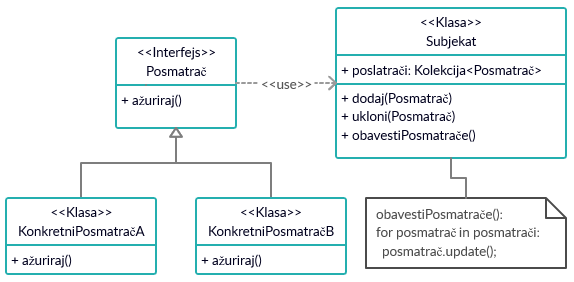
\includegraphics[scale=0.8]{images/design_observer.png}
\caption{UML dijagram obrasca za projektovanje "Posmatrač".}
\label{fig:UMLObserver}
\end{figure}

Primer upotrebe ovog obrasca može biti aukcija gde je aukcionar subjekat i započinje aukciju, dok učesnici aukcije (objekti) posmatraju aukcionera i reaguju na podizanje cene. Prihvatanje promene cene menja trenutnu cenu i aukcioner oglašava promenu iste, a svi učesnici aukcije dobijaju informaciju da se izmena izvršila. Za potrebe ovog rada, primer upotrebe može biti obilazak stablolike kolekcije (recimo stabla parsiranja) i obaveštavanje o nailasku na čvorove određenih tipova. Te informacije se dalje mogu iskoristiti za izračunavanja nad pomenutom strukturom ili generisanje novih struktura (recimo AST). 

\subsection{Obrazac "Posetilac"}
\label{subsec:DesignPatternsListener}

Obrazac za projektovanje \emph{Posetilac} je obrazac ponašanja koji predstavlja operaciju koju je potrebno izvesti nad elementima objektne strukture. Posetilac omogućava definisanje nove operacije bez izmena klasa elemenata nad kojima operiše. Operacija koja će se izvesti zavisi od imena zahteva, tipa posetioca i tipa elementa kog posećuje. Na slici \ref{fig:UMLVisitor} se može videti UML dijagram \cite{UML} ovog obrasca. 

\begin{figure}[h!]
    \centering
    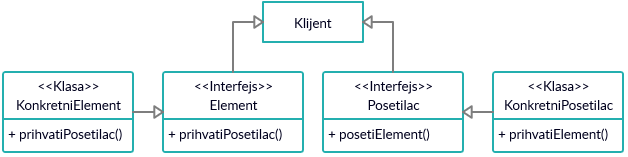
\includegraphics[scale=0.8]{images/design_visitor.png}
    \caption{UML dijagram obrasca za projektovanje "Posetilac".} 
    \label{fig:UMLVisitor}
\end{figure}

Primer upotrebe ovog obrasca može biti operisanje taksi kompanija. Kada osoba pozove taksi kompaniju (prihvatanje posetioca), kompanija šalje vozilo osobi koja je pozvala kompaniju. Nakon ulaska u vozilo (posetilac), mušterija ne kontroliše svoj transport već je to u rukama taksiste (posetioca). Za potrebe ovog rada, primer upotrebe može biti prikupljanje informacija o kolekciji stablolike strukture (recimo stablo parsiranja) i korišćenje istih za neko izračunavanje ili generisanje novih struktura (recimo AST). 

\section{Programske paradigme i gramatičke razlike programskih jezika}
\label{sec:Paradigms}

Iako se u suštini svode na mašinski jezik ili asembler, viši programski jezici mogu imati velike razlike međusobno --- kako u načinu pisanja koda, tako i u efikasnosti izvršavanja. Način, ili stil programiranja se naziva \emph{programska paradigma} \cite{ProgrammingParadigms}. Može se pokazati da sve što je rešivo putem jedne, može i da se reši i putem ostalih; međutim neki problemi se prirodnije rešavaju koristeći specifične paradigme. Neke poznatije programske paradigme su navedene u nastavku zajedno sa njihovim odlikama i primerima upotrebe.


\subsection{Imperativna paradigma}
\label{subsec:ParadigmImperative}

\emph{Imperativna paradigma} pretpostavlja da se promene u trenutnom stanju izvršavanja mogu sačuvati kroz promenljive. Izračunavanja se vrše putem niza koraka, u svakom koraku se te promenljive referišu ili se menjaju njihove trenutne vrednosti. Raspored koraka je bitan, jer svaki korak može imati različite posledice s obzirom na trenutne vrednosti promenljivih na početku tog koraka. Primer koda pisanog u imperativnoj paradigmi se može videti na slici \ref{fig:ParadigmImperative}.

\begin{figure}[h!]
\begin{lstlisting}
    result = []
    i = 0
start:
    numPeople = length(people)
    if i >= numPeople goto finished
    p = people[i]
    nameLength = length(p.name)
    if nameLength <= 5 goto nextOne
    upperName = toUpper(p.name)
    addToList(result, upperName)
nextOne:
    i = i + 1
    goto start
finished:
    return sort(result)
\end{lstlisting}
\caption{Primer koda pisanog u imperativnoj paradigmi.}
\label{fig:ParadigmImperative}
\end{figure}

Stariji programski jezici najčešće prate ovu paradigmu više nego bilo koju drugu iz par razloga. Prvi je taj što imperativna paradigma najbliže oslikava samu mašinu na kojoj se program izvršava, pa je programer mnogo "bliži" mašini. Ova paradigma je bila veoma popularna zbog ranih ograničenja u hardveru i potrebe za efikasnim programima. Danas, zbog mnogo bržeg razvoja i mnogo jačih računara, efikasnost se sve manje uzima u obzir.

Naravno, imperativna paradigma ima i svoje nedostatke. Naime, najveći problem je razumevanje i verifikovanje semantike programa zbog postojanja sporednih efekata\footnote{Sporedni efekti (promena stanja mašine) ne poštuju \emph{referencijalnu transparentnost} koja se definiše na sledeći način: \emph{Ako važi $P(x)$ i $x = y$ u nekom trenutku, onda $P(x) = P(y)$ važi tokom čitavog vremena izvršavanja programa}.}. Stoga je i pronalaženje grešaka u programima pisanim u imperativnoj paradigmi znatno komplikovanije. Pošto je k\^od veoma niskog nivoa, apstrakcija takvog koda je više ograničena nego u ostalim paradigmama. Na kraju, redosled izvršavanja je vrlo bitan, što neke probleme čini težim ukoliko se pokušaju rešiti pomoću imperativne paradigme.


\subsection{Strukturna paradigma}
\label{subsec:ParadigmImperativeStructural}

\emph{Strukturna paradigma} je vrsta imperativne paradigme gde se kontrola toka vrši putem ugnježdenih petlji, uslovnih grananja i podrutina. Promenljive su obično lokalne za blok u kome su definisane, što određuje i njihov životni vek i vidljivost. Primer koda pisanog u strukturnoj paradigmi se može videti na slici \ref{fig:ParadigmStructural}. Danas je najpopularnija kombinacija strukturne paradigme sa \emph{proceduralnom paradigmom}, baziranom na konceptu poziva \emph{procedure} --- podrutine ili funkcije koja sadrži seriju koraka koje je potrebno izvršiti redom.

\begin{figure}[h!]
\begin{lstlisting}
result = [];
for (i = 0; i < length(people); i++) {
    p = people[i];
    if (length(p.name)) > 5 {
        addToList(result, toUpper(p.name));
    }
}
return sort(result);
\end{lstlisting}
\caption{Primer koda pisanog po strukturnoj paradigmi.}
\label{fig:ParadigmStructural}
\end{figure}


\subsection{Skript paradigma i njen odnos sa proceduralnom paradigmom}
\label{subsec:Languages}

Čak i unutar jedne paradigme kao što je proceduralna, mogu se naći veoma velike varijacije u izgledu koda pisanog u različitim programskim jezicima koji prate proceduralnu paradigmu. Kako hardver postaje moćniji, više se ceni vreme koje programer provede u procesu pisanja koda nego koliko je taj kod efikasan. Štaviše, u nekim slučajevima je dobitak u efikasnosti veoma mali u poređenju sa vremenom koje je potrebno utrošiti da bi se ta efikasnost postigla. Ukoliko se program pokreće veoma retko, možda nije ni bitno da li se on izvršava sekundu sporije od efikasnog programa, ako je za njegovo pisanje utrošeno znatno manje vremena. Ovo je pristup koji prate \emph{skript} jezici kao što su \texttt{Python, Perl, bash} itd. Iako proceduralni, oni se razlikuju od klasičnih predstavnika proceduralne paradigme i njihove razlike su vremenom postale tolike da nije neuobičajeno da se skript jezici svrstaju u zasebnu, \emph{skript paradigmu}. Stoga će se u nastavku, pod terminom \emph{proceduralni jezik} smatrati tradicionalni proceduralni jezik, ukoliko nije naznačeno drugačije. Na slici \ref{fig:LanguagesDiff} se mogu uočiti navedene razlike.

\begin{figure}[h!]
\begin{lstlisting}
int main() {
    int k = 0;
    for (int i = 0; i < 1000000; i++)
        k++;
    return 0;
}
\end{lstlisting}
\begin{lstlisting}[language={}]
$ time: 0.03s user 0.00s system 70% cpu 0.044 total
\end{lstlisting}
\begin{lstlisting}
k = 0
for i in range(1000000):
    k += 1
\end{lstlisting}
\begin{lstlisting}[language={}]
$ time: 0.16s user 0.03s system 93% cpu 0.200 total
\end{lstlisting}
\caption{Primer koda pisanog po tradicionalnoj proceduralnoj paradigmi (gore, \texttt{C}) i po modernoj skript paradigmi (dole, \texttt{Python 3}) kao i odgovarajuća vremena izvršavanja dobijena komandom \texttt{time}.}
\label{fig:LanguagesDiff}
\end{figure}

Promenljive predstavljaju jedan od osnovnih koncepata na kojem se zasnivaju i proceduralni i skript jezici. Promenljivu odlikuje, između ostalog, i njen \emph{tip} koji određuje količinu memorije potrebnu za njeno skladištenje. Proceduralni programski jezici zahtevaju definisanje tipa promenljive i obično su i \emph{statički}, što znači da promenljive ne mogu menjati svoj tip tokom izvršavanja programa. Proces uvođenja imena promenljive se u naziva \emph{deklaracija promenljive}. Slično kao i za promenljive, potrebno je deklarisati i funkcije pre trenutka njihovog korišćenja kako bi prevodilac znao broj i tipove parametara funkcije kao i njihove povratne vrednosti. Skript jezici žrtvuju statičku tipiziranost kako bi proces pisanja koda bio brži. Stoga su oni obično \emph{dinamički} --- promenljive mogu menjati tip tokom izvršavanja programa. Pošto promenljive mogu menjati svoj tip, definisanje tipa prilikom uvođenja imena promenljive postaje redundantno jer prevodilac može to sam da zaključi. Stoga i sam proces uvođenja imena promenljive postaje redundantan. Slično, parametri funkcija takođe nisu fiksnog tipa. Slično važi i za povratnu vrednost funkcije.

Kod proceduralnih jezika, pošto su obično statički tipizirani, mogu se iskoristiti strukture podataka koje omogućavaju brz pristup svojim elementiram. To su obično nizovi koji predstavljaju kontinualni blok memorije u kom su elementi niza smešteni jedan do drugog. Pristup se vrši na osnovu indeksa i, pošto su svi elementi istog tipa (zauzimaju jednaku količinu memorije), može se u konstantnom vremenu izračunati memorijska lokacija na kojoj se nalazi element niza sa datim indeksom. Kompleksnije strukture podataka obično nisu podržane u samom jeziku. Neki proceduralni jezici dozvoljavaju veoma niski pristup kroz \emph{pokazivače} ili \emph{reference} na memorijske adrese (\texttt{C} i \texttt{C++}). Većina modernih proceduralnih jezika ne dozvoljava rad sa pokazivačima, ne brinući puno o efikasnosti, dok neki dozvoljavaju korišćenje pokazivača u specijalnim situacijama sa eksplicitnom naznakom (\texttt{C\#}).

Pored dinamičnosti kad je u pitanju tip promenljivih, skript jezici često imaju neke specifične strukture podataka ugrađene u sam jezik kao olakšice prilikom programiranja. Primarna struktura podataka je \emph{jednostruko ulančana lista}\footnote{Lista je rekurzivna kolekcija podataka koja se sastoji od glave koja sadrži vrednost određenog tipa, i pokazivača na rep --- drugu listu. Specijalno, praznim pokazivačima se označava kraj liste (prazna lista).}, za razliku od niza kod proceduralnih jezika. Razlog zašto se koriste liste je delimično zbog toga što, kao i ostale promenljive, liste ne moraju da budu statički tipizirane. Moguće je u listu ubacivati elemente različitih tipova --- što onemogućava skladištenje u kontinualnom bloku memorije (osim ukoliko je lista imutabilna, što nije obično slučaj). Skript jezici uglavnom omogućavaju indeksni pristup elementima liste pa programeru izgleda kao da radi nad običnim nizom. Neki skript jezici omogućavaju kreiranje \emph{asocijativnih nizova}, gde indeks niza ne mora biti ceo broj već može uzimati vrednost iz domena bilo kog tipa. Osim listi, obično su podržane i torke, i za njih važe iste slobode kao i za liste. Kompleksnije strukture podataka uključuju skupove i rečnike (drugačije nazivane i \emph{heš mape}, engl. \emph{hash map}) koji su kolekcija ključ-vrednost parova gde je dozvoljen indeksni pristup po vrednosti ključa. Skript programski jezici su skoro uvek interpretirani, iako se neki jezici mogu kompajlirati po potrebi za efikasnije ponovno izvršavanje. S obzirom da efikasnost nije u glavnom planu, u skript jezicima nije dozvoljen direktan pristup memoriji putem pokazivača ili referenci. 


\subsection{Ostale popularne programske paradigme}
\label{subsec:ParadigmsOther}

\emph{Objektno-orijentisana paradigma} (kraće \emph{OOP}) je paradigma u kojoj se objekti stvarnog sveta posmatraju kao zasebni entiteti koji imaju sopstveno stanje koje se modifikuje samo pomoću procedura ugrađenih u same objekte --- tzv. \emph{metode}. Posledica zasebnog operisanja objekata omogućava njihovu enkapsulaciju u module koji sadrže lokalnu sredinu i metode. Komunikacija sa objektom se vrši prosleđivanjem poruka. Objekti su organizovani u klase, od kojih nasleđuju atribute i metode. OOP omogućava ponovnu iskorišćenost koda i ekstenzibilnost koda.

\emph{Logička paradigma} koristi deklarativni pristup rešavanju problema. Umesto zadavanja instrukcija koje treba da dovedu do rezultata, opisuje se sam rezultat kroz činjenice --- skup logičkih pretpostavki koji se zatim prevodi u upit koji se dalje koristi. Uloga računara je održavanje i logička dedukcija.

\emph{Funkcionalna paradigma} posmatra sve potprograme kao funkcije u matematičkom smislu --- uzimaju argumente i vraćaju jedinstven rezultat. Povratna vrednost zavisi isključivo od argumenata, što znači da je nebitan trenutak u kom je funkcija pozvana. Izračunavanja se vrše primenom i kompozicijom funkcija. 


\chapter{Opis opšte AST apstrakcije za imperativne jezike}
\label{chp:MyAST}

U ovom poglavlju će biti opisane sličnosti i razlike koncepata pruženih od strane raznih programskih jezika kao i opis apstrakcije za koncepte zajedničke za imperativne programske jezike. U odeljku \ref{sec:Paradigms} će biti opisane "grupe" programskih jezika na osnovu sličnosti u načinu pisanja koda u tim programskim jezicima, dok će u odeljku \ref{sec:MyAST} biti više reči o apstrakciji za imperativne programske jezike.

\section{Programske paradigme}
\label{sec:Paradigms}

Iako se u suštini svode na mašinski jezik ili asembler, viši programski jezici mogu imati velike razlike međusobno --- kako u načinu pisanja koda, tako i u efikasnosti izvršavanja. Način, ili stil programiranja se naziva \emph{programska paradigma} \cite{ProgrammingParadigms}. Može se pokazati da sve što je rešivo putem jedne, može da se reši i putem ostalih; međutim neki problemi se prirodnije rešavaju koristeći specifične paradigme. Neke poznatije programske paradigme su navedene u nastavku zajedno sa njihovim odlikama i primerima upotrebe.


\subsection{Imperativna paradigma}
\label{subsec:ParadigmImperative}

\emph{Imperativna paradigma} pretpostavlja da se promene u trenutnom stanju izvršavanja mogu sačuvati kroz promenljive. Izračunavanja se vrše putem niza koraka, u svakom koraku se te promenljive referišu ili se menjaju njihove trenutne vrednosti. Raspored koraka je bitan, jer svaki korak može imati različite posledice s obzirom na trenutne vrednosti promenljivih na početku tog koraka. Primer koda pisanog u imperativnoj paradigmi se može videti na slici \ref{fig:ParadigmImperative}.

\begin{figure}[h!]
\begin{lstlisting}
    result = []
    i = 0
start:
    numPeople = length(people)
    if i >= numPeople goto finished
    p = people[i]
    nameLength = length(p.name)
    if nameLength <= 5 goto nextOne
    upperName = toUpper(p.name)
    addToList(result, upperName)
nextOne:
    i = i + 1
    goto start
finished:
    return sort(result)
\end{lstlisting}
\caption{Primer koda pisanog u imperativnoj paradigmi.}
\label{fig:ParadigmImperative}
\end{figure}

Stariji programski jezici najčešće prate ovu paradigmu iz nekoliko razloga. Prvi je taj što imperativna paradigma najbliže oslikava samu mašinu na kojoj se program izvršava, pa je programer mnogo bliži mašini. Ova paradigma je bila veoma popularna zbog ranih ograničenja u hardveru i potrebe za efikasnim programima. Danas, zbog mnogo bržeg razvoja i mnogo jačih računara, efikasnost dobijena pisanjem koda u jezicima veoma bliskim mašini se sve manje uzima u obzir.

Imperativna paradigma svoje nedostatke. Naime, najveći problem je razumevanje i verifikovanje ispravnosti programa zbog postojanja propratnih efekata\footnote{Propratni efekti (promena stanja mašine) ne poštuju \emph{referencijalnu transparentnost} koja se definiše na sledeći način: \emph{Ako važi $P(x)$ i $x = y$ u nekom trenutku, onda $P(x) = P(y)$ važi tokom čitavog vremena izvršavanja programa}.}. Stoga je zahtevno i pronalaženje grešaka u programima pisanim u imperativnoj paradigmi. Pošto je k\^od veoma niskog nivoa, obično je dozvoljen i direktan pristup memorijskim adresama putem \emph{pokazivača}, što takođe otežava verifikaciju koda.


\subsection{Strukturna paradigma}
\label{subsec:ParadigmImperativeStructural}

\emph{Strukturna paradigma} je vrsta imperativne paradigme gde se kontrola toka vrši putem niza naredbi, uslovnih grananja i petlji. Promenljive su obično lokalne za blok u kome su definisane, što određuje i njihov životni vek i vidljivost. Primer koda pisanog u strukturnoj paradigmi se može videti na slici \ref{fig:ParadigmStructural}. Danas je najpopularnija kombinacija strukturne paradigme sa \emph{proceduralnom paradigmom}, baziranom na konceptu poziva \emph{procedure} --- podrutine ili funkcije koja sadrži seriju koraka koje je potrebno izvršiti redom.

\begin{figure}[h!]
\begin{lstlisting}
result = [];
for (i = 0; i < length(people); i++) {
    p = people[i];
    if (length(p.name)) > 5 {
        addToList(result, toUpper(p.name));
    }
}
return sort(result);
\end{lstlisting}
\caption{Primer koda pisanog u strukturnoj paradigmi.}
\label{fig:ParadigmStructural}
\end{figure}


\subsection{Skript paradigma i njen odnos sa proceduralnom paradigmom}
\label{subsec:Languages}

Čak i unutar jedne paradigme kao što je proceduralna, mogu se naći veoma velike varijacije u izgledu koda pisanog u različitim programskim jezicima. Kako hardver postaje moćniji, više se ceni vreme koje programer provede u procesu pisanja koda nego koliko je taj k\^od efikasan. Štaviše, u nekim slučajevima je dobitak u efikasnosti veoma mali u poređenju sa vremenom koje je potrebno utrošiti da bi se ta efikasnost postigla. Ukoliko se program pokreće veoma retko, možda nije ni bitno da li se on izvršava sekundu sporije od efikasnog programa, ako je za njegovo pisanje utrošeno znatno manje vremena. Ovo je pristup koji prate \emph{skript} jezici kao što su \texttt{Python, Lua, Perl, bash} itd. Iako proceduralni, oni se razlikuju od klasičnih predstavnika proceduralne paradigme i njihove razlike su vremenom postale tolike da se skript jezici obično svrstavaju u zasebnu, \emph{skript paradigmu}. Stoga će se u nastavku pod terminom \emph{proceduralni jezik} smatrati tradicionalni proceduralni jezik, ukoliko nije naznačeno drugačije. Na slici \ref{fig:LanguagesDiff} se mogu uočiti navedene razlike.

\begin{figure}[h!]
\begin{lstlisting}
int main() {
    int k = 0;
    for (int i = 0; i < 1000000; i++)
        k++;
    return 0;
}
\end{lstlisting}
\begin{lstlisting}[language={}]
$ time: 0.03s user 0.00s system 70% cpu 0.044 total
\end{lstlisting}
\begin{lstlisting}
k = 0
for i = 0, 1000000 do 
    k = k + 1 
end
\end{lstlisting}
\begin{lstlisting}[language={}]
$ time: 0.17s user 0.03s system 92% cpu 0.203 total
\end{lstlisting}
\caption{Primer koda pisanog u tradicionalnoj proceduralnoj paradigmi (gore, \texttt{C}) i u modernoj skript paradigmi (dole, \texttt{Lua}) kao i odgovarajuća vremena izvršavanja dobijena komandom \texttt{time}.}
\label{fig:LanguagesDiff}
\end{figure}

Promenljive predstavljaju jedan od osnovnih koncepata na kojem se zasnivaju i proceduralni i skript jezici. Promenljivu odlikuje, između ostalog, i njen \emph{tip} koji određuje količinu memorije potrebnu za njeno skladištenje. Proceduralni programski jezici najčešće zahtevaju eksplicitno definisanje tipa promenljive u kodu jer su većinom \emph{statički tipizirani}, što znači da se tipovi promenljivih određuju u fazi prevođenja --- posledica toga je da promenljive ne mogu menjati svoj tip tokom izvršavanja programa. Proces uvođenja imena za memorijsku lokaciju koja predstavlja mesto skladištenja vrednosti promenljive određenog tipa se naziva \emph{deklaracija promenljive}. Slično kao i za promenljive, potrebno je deklarisati i funkcije pre trenutka njihovog korišćenja kako bi prevodilac znao broj i tipove parametara funkcije kao i njihove povratne vrednosti. Skript jezici su, za razliku od proceduralnih, najčešće \emph{dinamički tipizirani}, što znači da tipovi promenljivih zavise od trenutnih vrednosti promenljviih u fazi izvršavanja. Stoga je proces pisanja koda u dinamički tipiziranim jezicima brži jer se ne moraju navesti tipovi promenljivih\footnote{U nekim programskim jezicima koji su statički tipizirani (npr.~Haskell) prevodilac može da zaključi tip na osnovu konteksta u kom se promenljiva koristi, stoga programer ne mora da eksplicitno navede tipove funkcija. Takođe, većina skript jezika dozvoljava eksplicitno definisanje tipa, ali to nije neophodno da bi se k\^od preveo.}. Slično, parametri i povratne vrednosti funkcija takođe ne moraju biti fiksnog tipa.

Kod statički tipiziranih proceduralnih jezika, mogu se koristiti strukture podataka koje omogućavaju brz pristup svojim elementima. To su na primer nizovi koji predstavljaju kontinualni blok memorije u kom su elementi niza smešteni jedan do drugog. Pristup se vrši na osnovu indeksa i, pošto su svi elementi istog tipa (zauzimaju jednaku količinu memorije), može se u konstantnom vremenu izračunati memorijska lokacija na kojoj se nalazi element niza sa datim indeksom. Kompleksnije strukture podataka obično nisu podržane u samom jeziku. Neki proceduralni jezici dozvoljavaju veoma niski pristup kroz \emph{pokazivače} ili \emph{reference} na memorijske adrese (npr. \texttt{C}, \texttt{C++}, \texttt{Go}, \texttt{Rust}). Većina modernih proceduralnih jezika (npr. \texttt{Java}, \texttt{JavaScript}. \texttt{Python}, \texttt{Lua}) ne dozvoljava korišćenje pokazivača, dok neki to dozvoljavaju ali sa eksplicitnom naznakom (\texttt{C\#}).

Pored dinamičnosti kad je u pitanju tip promenljivih, skript jezici često imaju neke specifične strukture podataka ugrađene u sam jezik kao olakšice prilikom programiranja. Za razliku od proceduralnih jezika gde su osnovne strukture podataka često kontinualni blokovi memorije sa proizvoljnim pristupom po indeksu, primarna struktura podataka kod skript jezika je najčešće \emph{jednostruko ulančana lista}\footnote{Lista je rekurzivna kolekcija podataka koja se sastoji od glave koja sadrži vrednost određenog tipa, i pokazivača na rep --- drugu listu. Specijalno, praznim pokazivačima se označava kraj liste (prazna lista).}. Razlog zašto se koriste liste je delimično zbog toga što, kao i ostale promenljive, liste ne moraju da budu statički tipizirane. Moguće je u listu ubacivati elemente različitih tipova --- što onemogućava skladištenje u kontinualnom bloku memorije (osim ukoliko je lista nepromenljiva, što obično nije slučaj). Skript jezici uglavnom omogućavaju indeksni pristup elementima liste, pa programeru izgleda kao da radi nad običnim nizom. Neki skript jezici omogućavaju kreiranje \emph{asocijativnih nizova}, gde indeks niza ne mora biti ceo broj već može uzimati vrednost iz domena bilo kog tipa. Osim listi, obično su podržane i \texttt{torke}\footnote{Torka (engl. \emph{tuple}) je nepromenljiva, uređena struktura podataka koja predstavlja sekvencu elemenata.}, i za njih važe iste slobode kao i za liste. Kompleksnije strukture podataka uključuju skupove i rečnike ili \emph{mape} (engl. \emph{dictionaries, maps}) koji predstavljau kolekciju ključ-vrednost parova gde je dozvoljen indeksni pristup vrednosti para koristeći ključ. Razne implementacije mapa postoje i u proceduralnim jezicima, ali ključna razlika je ta što tipovi u skript jezicima nisu striktni --- ključevi međusobno, ali i vrednosti mogu biti različitog tipa. Vredi naglasiti da se mape mogu porediti sa objektima određenih klasa --- svaki objekat se može serijalizovati u mapu gde su ključevi imena javnih atributa klase a vrednosti su vrednosti javnih atributa objekta koji se serijalizuje. Neki jezici (kao što je Python), imaju funkcije koje od objekta vraćaju baš ovakvu mapu. U programskom jeziku Lua, asocijativni nizovi (tzv. \emph{tabele}) implementiraju sve ostale strukture podatake, pa i klase, što direktno odgovara ideji poređenja objekata sa rečnicima odnosno asocijativnim nizovima.

Skript programski jezici su skoro uvek interpretirani, iako se neki jezici mogu kompilirati po potrebi za efikasnije ponovno izvršavanje. S obzirom da efikasnost nije u glavnom planu, u skript jezicima nije dozvoljen direktan pristup memoriji putem pokazivača ili referenci. 


\subsection{OO paradigma i njen odnos sa proceduralnom paradigmom}
\label{subsec:ParadigmOOP}

\emph{Objektno-orijentisana paradigma} (kraće \emph{OOP} ili \emph{OO paradigma}) je paradigma u kojoj se objekti stvarnog sveta posmatraju kao zasebni entiteti koji imaju sopstveno stanje koje se modifikuje samo pomoću procedura ugrađenih u same objekte --- tzv. \emph{metode}. Pošto objekti operišu nezavisno jedni od drugih, moguće je enkapsulirati ih u module koji sadrže lokalnu sredinu i metode dok se komunikacija sa objektom vrši prosleđivanjem poruka. Objekti su organizovani u klase, od kojih nasleđuju atribute i metode. OO paradigma omogućava ponovno korišćenje i jednostavnu proširivost koda. Primer koda pisanog u OO paradigmi se može videti na slici \ref{fig:ParadigmOO}.

\begin{figure}[h!]
\begin{lstlisting}
class Person
{
    private string name;
    private int wage;
    private int income = 0;

    Person(string name, int wage) {
        this.name = name;
        this.wage = wage;
    }

    public void Work(int hours) {
        this.income += hours * this.wage;
    }
}

Person p1 = new Person("John Doe", 30);
Person p2 = new Person("Dave Doe", 35);
p1.Work(7);
p2.Work(8);
\end{lstlisting}
\caption{Primer koda pisanog u OO paradigmi.}
\label{fig:ParadigmOO}
\end{figure}

Iako se OOP posmatra kao zasebna paradigma, moderni programski jezici često koriste OO koncepte iako nisu nužno predstavnici OO paradigme. Jedan od primera je i programski jezik \texttt{Python} koji, iako svrstan u skript paradigmu, pruža i OO koncepte kao što su klase, metode i nasleđivanje. Razlog za ovo je najviše prednost koje OO paradigma pruža ukoliko se radi na velikim programima, ali i taj što implementacija metoda OO klasa podseća na proceduralni k\^od. Neki programski jezici kao što je \texttt{Lua} nemaju koncept klase, ali imaju koncept nasleđivanja. U ovom radu neće biti implementirane apstrakcije OO koncepata kao što su klase ili interfejsi.

\subsection{Ostale popularne programske paradigme}
\label{subsec:ParadigmsOther}

\emph{Logička paradigma} koristi deklarativni pristup rešavanju problema i po tome se razlikuje od ostalih paradigmi opisanih u ovom odeljku. Umesto zadavanja instrukcija koje treba da dovedu do rezultata, opisuje se sam rezultat kroz činjenice --- skup logičkih pretpostavki koji se zatim prevodi u upit koji se dalje koristi. Uloga računara je održavanje skupa poznatih činjenica i logička dedukcija korišćenjem skupa poznatih činjenica iz koje proizilaze nove činjenice koje su od značaja za rešavanje problema. 

\emph{Funkcionalna paradigma} posmatra sve potprograme kao funkcije u matematičkom smislu --- uzimaju argumente i vraćaju jedinstven rezultat. Povratna vrednost zavisi isključivo od argumenata, što znači da je nebitan trenutak u kom je funkcija pozvana. Izračunavanja se vrše primenom i kompozicijom funkcija. Strukture podataka su nepromenljive i mogu biti beskonačne jer se izračunavanje elemenata kolekcija može vršiti po potrebi (npr. u programskom jeziku Haskell). Poštovanje referencijalne transparentnosti i nepromenljivost struktura podataka ima za posledicu da se k\^od može implicitno paralelizovati ali i lakše verifikovati njegova ispravnost. Takođe, programi pisani u funkcionalnoj paradigmi komponovanjem funkcija višeg reda su često veoma čitljivi i kratki. Zbog svojih prednosti, funkcionalni koncepti se često uključuju u moderne predstavnike proceduralne paradigme (npr. \texttt{C++}, \texttt{Java}, \texttt{C\#}, \texttt{Python}, \texttt{Lua}). Iako je u ovom radu akcenat na imperativnoj paradigmi, neki funkcionalni koncepti su implicitno podržani zbog načina na koji je implementiran opšti AST --- operatori kompozicije funkcija, funkcije višeg reda i anonimne funkcije. Sa druge strane, poređenje funkcionalnog koda sa imperativnim kodom nije razmatrano. 

\section{Opšte apstraktno sintaksičko stablo}
\label{sec:MyAST}

Kao što je opisano u odeljku \ref{sec:Paradigms}, dosta različitih "pod-paradigmi" potiče iz imperativne paradigme. Strukturna, proceduralna i skript paradigma, iako naizgled različite, poseduju veliki broj sličnih osobina i koncepata. Moderni programski jezici uzimaju korisne koncepte iz svakakvih paradigmi pa je teško vezati jezik za jednu konkretnu paradigmu. Ovo je motivacija za apstrahovanje koncepata različitih paradigmi, ali pre svega imperativne i njenih "derivata" --- proceduralne, skript i objektno orijentisane. U ovom poglavlju će biti opisana opšta apstrakcija za imperativnu paradigmu i njene derivate. To uključuje i skript jezike koji, kako će biti pokazano u ovom radu, mogu da se posmatraju na istom nivou kao i svoji proceduralni "rođaci".

Svaki programski jezik ima svoju gramatiku i na osnovu toga ima svoja gramatička pravila koja se oslikavaju u apstraktnim sintaksnim stablima tih jezika. Na slikama \ref{fig:ASTLua} i \ref{fig:ASTGo} se mogu videti razlike jezika \texttt{Lua} i \texttt{Go}, kao primere skript odnosno proceduralne paradigme, kad se posmatra njihov AST.

\begin{figure}[h!]
\centering
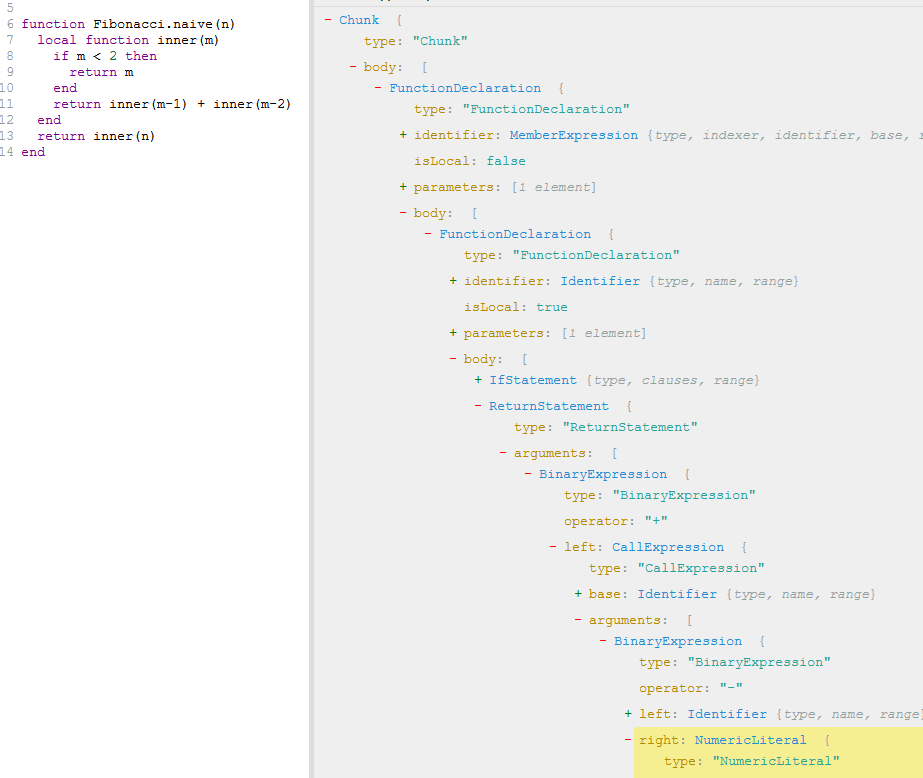
\includegraphics[scale=0.6]{images/ast_lua.png}
\caption{AST isečka koda pisanog u programskom jeziku Lua. Prikazano putem \url{https://astexplorer.net/}}
\label{fig:ASTLua}
\end{figure}

\begin{figure}[h!]
\centering
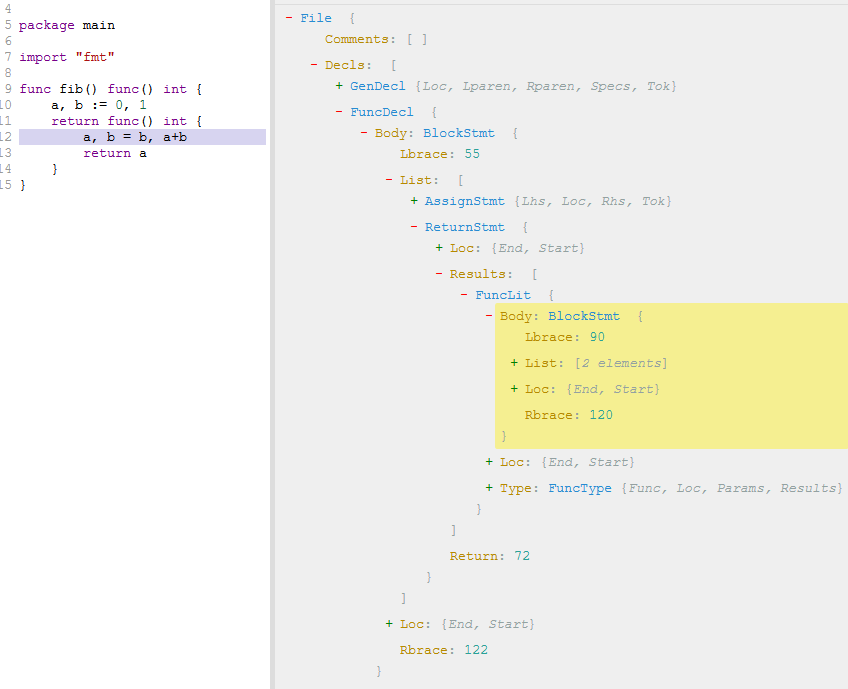
\includegraphics[scale=0.7]{images/ast_go.png}
\caption{AST isečka koda pisanog u programskom jeziku Go. Prikazano putem \url{https://astexplorer.net/}}
\label{fig:ASTGo}
\end{figure}

Kako bi se kreirala smislena apstrakcija stabla parsiranja, potrebno je identifikovati bitne informacije u stablu parsiranja ali i koncepte same gramatike koji su ponovno upotrebljivi. Najjednostavnije rešenje je mimikovati čvorove stabla parsiranja, ukoliko su gramatička pravila kreirana tako da oslikaju koncepte jezika koji gramatika definiše. Na primer, ukoliko u gramatici imamo pravilo \texttt{deklaracija} sa alternativama \texttt{deklaracijaPromenljive} i \texttt{deklaracijaFunkcije}, možemo kreirati apstraktni koncept \texttt{Deklaracija} sa konkretizacijama \texttt{DeklaracijaPromenljive} i \texttt{DeklaracijaFunkcije}. Kako se definišu deklaracije promenljivih i funkcija zavisi dalje od definicija pravila \texttt{deklaracijaPromenljive} i \texttt{deklaracijaFunkcije}. Naravno, nije uvek moguće primeniti ovakav postupak. Takođe, nekada u gramatici definišemo pomoćna pravila kako bismo se izborili sa rekurzijom ili izbegli neke tipove rekurzije --- ta pravila ne bi trebalo da imaju odgovarajuće tipove u opštoj apstrakciji. 

Pošto su u pitanju gramatike programskih jezika, onda je jasno da dosta različitih gramatika dele slične koncepte i da je moguće definisati tipove čvorova koji odgovaraju tim konceptima. Neki od njih mogu biti: naredba, izraz, deklaracija, poziv funkcije, dodela itd. Može se uočiti i hijerarhija između navedenih koncepata, međutim poziv funkcije se može smatrati kao samostalna naredba ali može biti i deo izraza. Dakle, prilikom definisanja hijerarhije ne treba dozvoliti nešto što nema smisla (npr. ako je dozvoljeno višestruko nasleđivanje i poziv funkcije je i naredba ali i izraz, onda se izrazi u kojima figurišu pozivi funkcija sastoje od više naredbi.).

Osim naredbi i izraza (koje vezuju operatori), kao osnovnih koncepata imperativnih jezika, deklaracije se ne pojavljuju u skript jezicima zbog slabe tipiziranosti. Moguće je, međutim, posmatrati i promenljive u kodovima skript jezika kao promenljive deklarisane neposredno pre trenutka njihove upotrebe --- detaljnije opisano u \ref{subsec:MyASTDeclarationNodes}. Što se tiče njihovog tipa, može biti dozvoljena promena istog, ili, kako je izabrano u ovom radu, biće iskorišćen specijalni tip od kog potiču svi ostali tipovi.

\begin{figure}[h!]
\centering
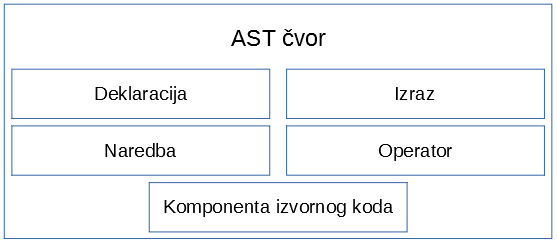
\includegraphics[scale=0.6]{images/nodes.png}
\caption{Prikaz osnovnih vrsta AST čvorova.}
\label{fig:ASTNode}
\end{figure}

Na slici \ref{fig:ASTNode} se mogu videti osnovni tipovi AST čvorova zasnovani na konceptima opisanim iznad. U nastavku će po odeljcima biti detaljnije opisan svaki od prikazanih tipova.

\subsection{Čvorovi deklaracija}
\label{subsec:MyASTDeclarationNodes}

Kao što je opisano u odeljku \ref{sec:Paradigms}, u striktno tipiziranim proceduralnim jezicima promenljive i funkcije koje se koriste se moraju deklarisati pre trenutka njihovog korišćenja. Prateći kvalifikatori (statičnost, konstantnost itd.) i modifikatori pristupa (javni, privatni itd.) će se u nastavku nazivati \emph{specifikatori deklaracije} (engl. \emph{declaration specifiers}). Nakon specifikatora deklaracije dolazi konkretan \emph{deklarator}, koji ima specifičan oblik u zavisnosti od toga šta se deklariše. Oba imena su uzeta po uzoru na imena pravila gramatike programskog jezika C. 

Veliki broj proceduralnih jezika dozvoljava deklarisanje više promenljivih odjednom koje dele iste specifikatore deklaracije. Stoga specifikatore neće pratiti jedan deklarator, nego \emph{lista deklaratora}. Takođe, deklaratori u listi ne moraju biti samo deklaratori promenljivih --- moguće je deklarisati i nizovnu promenljivu zajedno sa deklaracijama običnih promenljivih. Na slici \ref{fig:DeclarationParts} se može videti dekompozicija deklaracije promenljive i niza u različitim proceduralnim programskim jezicima a na slici \ref{fig:DeclarationNodes} uočena hijerarhija sa podvrstama deklaratora.

\begin{figure}[h!]
\centering
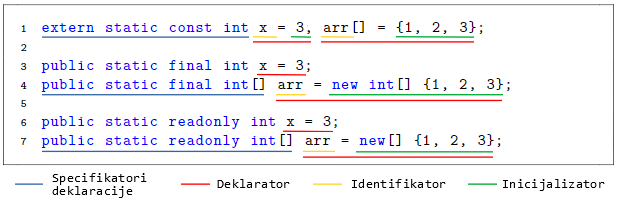
\includegraphics[scale=0.8]{images/declaration_decomposition.png}
\caption{Delovi deklaracije promenljive i niza prikazani na isečcima koda pisanog u programskim jezicima C, Java i C\#.}
\label{fig:DeclarationParts}
\end{figure}

\begin{figure}[h!]
\centering
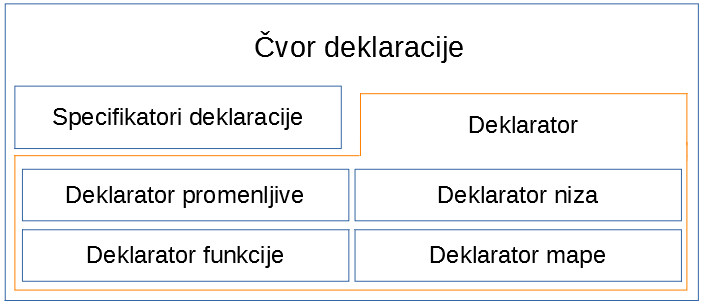
\includegraphics[scale=0.5]{images/declaration_nodes.png}
\caption{Prikaz vrsti AST čvorova deklaracije.}
\label{fig:DeclarationNodes}
\end{figure}

Kao što je prikazano na slici \ref{fig:DeclarationParts}, specifikatori deklaracije pokrivaju kvalifikatore, specifikatore pristupa i ime tipa. Pošto se pravi zajednička apstrakcija, potrebno je uočiti ekvivalenetne ključne reči u različitim programskim jezicima --- u primeru sa slike to su \texttt{const}, \texttt{final} i \texttt{readonly}. Imena tipova u programskim jezicima Java i C\# uzeta su po uzoru na programski jezik C, tako da tu ne vidimo razlike. U opštem slučaju, moguće je definisati mapiranje imena tipa u apstraktni tip. Ukoliko, na primer, posmatramo tipove koji predstavljaju realne brojeve, osim tipova \texttt{float} i \texttt{double}, postoji i tip \texttt{decimal}\footnote{Tip \texttt{decimal} predstavlja 128-bitni realan broj sa povećanom veličinom mantise a smanjenom veličinom eksponenta u odnosu na tip \texttt{double}. Koristi se pri numeričkm izračunavanjima gde preciznost primitivnih tipova realnih brojeva nije dovoljna.} prisutan u programskom jeziku C\#. Sva tri ova tipa mogu da se posmatraju na istom nivou apstrakcije kao tip realnih brojeva. Za korisnički definisane tipove isto ne može da se primeni.

Deklaratori za proceduralne jezike mogu biti deklaratori promenljive, niza ili funkcije i od toga zavisi njihov sastav. Svi deklaratori moraju sadržati informaciju o idenfitikatoru. Ukoliko je reč o deklaratoru niza, dodatno se očekuje i oznaka za niz (obično par srednjih zagrada --- \texttt{[]}) i opcioni izraz koji predstavlja dimenziju niza, obično unutar oznake niza. Ukoliko je reč o deklaratoru funkcije, pored identifikatora se očekuje i lista parametara funkcije obično navedena unutar para običnih zagrada. Lista parametara funkcije se može posmatrati rekurzivno --- svaki parametar se može posmatrati kao varijanta deklaracije --- sadrži specifikatore deklaracije (koji uključuju i tip) i deklarator, s tim što u ovom slučaju nije dozvoljeno da taj deklarator bude deklarator funkcije (pošto funkcije nisu građani prvog reda u imperativnoj paradigmi). 

Deklaratori promenljive i niza mogu dodatno sadržati i \emph{inicijalizator}. Inicijalizator možemo posmatrati kao opcioni izraz u slučaju deklaratora promenljive. U slučaju deklaratora niza, inicijalizator može biti lista izraza. Deklaratori funkcije ne mogu imati inicijalizatore.

U skript jezicima su uobičajeno podržane strukture podataka kao što su skupovi i mape. Stoga, kako bi se i mape mogle predstaviti apstraktno, dodat je tip deklaratora koji predstavlja deklarator mape. Mapa se sastoji od skupa ključeva pri čemu je svakom ključu dodeljena vrednost ne nužno istog tipa kao što je tip ključa. Mape postoje i u proceduralnim jezicima, ali ključna razlika je ta što tipovi u skript jezicima nisu striktni --- ključevi međusobno, ali i vrednosti mogu biti različitog tipa. Vredi naglasiti da se mape mogu porediti sa objektima određenih klasa --- svaki objekat se može serijalizovati u mapu gde su ključevi imena javnih atributa klase a vrednosti su vrednosti javnih atributa objekta koji se serijalizuje. Neki jezici (kao što je Python), imaju funkcije koje od objekta vraćaju baš ovakvu mapu. Ova ideja se dalje može proširiti kako bi se serijalizovale i metode klase, označila statička i privatna polja kao i sačuvale informacije o definisanim konstruktorima. Zatim je moguće porediti mape definisane u skript jezicima sa objektima iz proceduralnih jezika.

Na slici \ref{fig:MyASTExampleCDeclaration} se mogu videti kreirani AST za nekoliko deklaracija pisanih u programskom jeziku C a na slici \ref{fig:MyASTExampleLuaDeclaration} se može isto videti demonstracija \emph{automatske deklaracije} promenljivih za skript programski jezik Lua. Naime, pre prvog pojavljivanja identifikatora veštački će biti deklarisan taj identifikator, kako bi razlika između apstrakcija dobijenih iz proceduralnih i skript jezika bila što manja. U ovom slučaju će se deklaracija i dodela spojiti u deklaraciju sa inicijalizatorom.

\begin{figure}[h!]
\begin{lstlisting}
extern int y = 3;
static int arr[5] = { 1 };
\end{lstlisting}
\centering
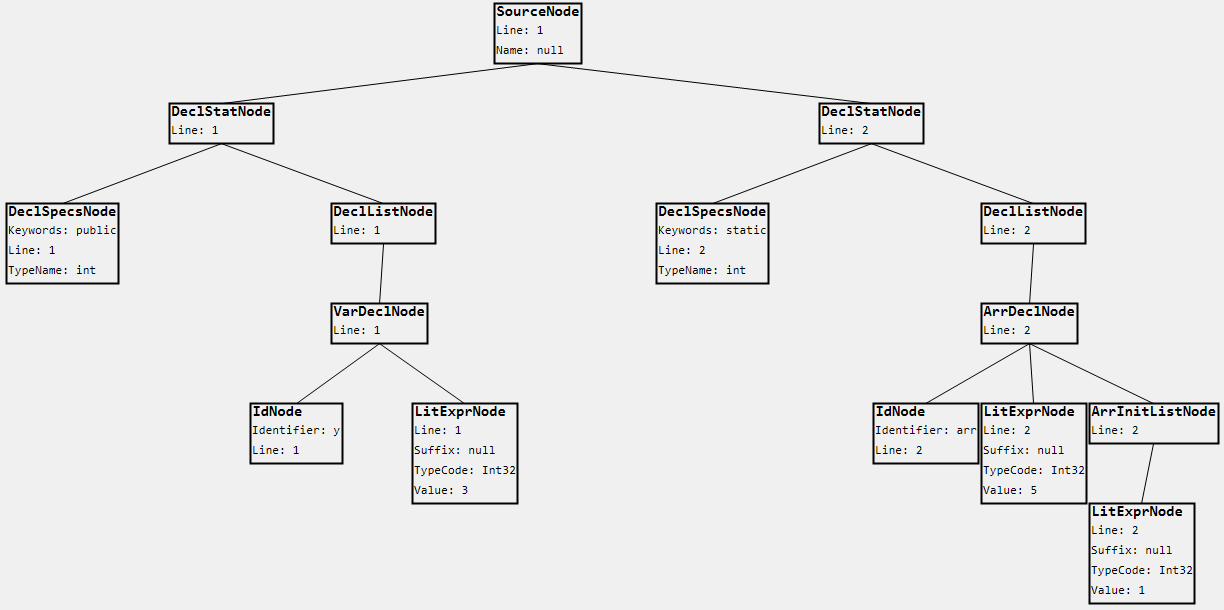
\includegraphics[scale=0.48]{images/c_ast_decl2.png}
\caption{Primer deklaracije promenljive i niza u programskom jeziku C i odgovarajući AST.}
\label{fig:MyASTExampleCDeclaration}
\end{figure}

\begin{figure}[h!]
\begin{lstlisting}
arr = { 1, 2 }
dict = { a = 1 }
\end{lstlisting}
\centering
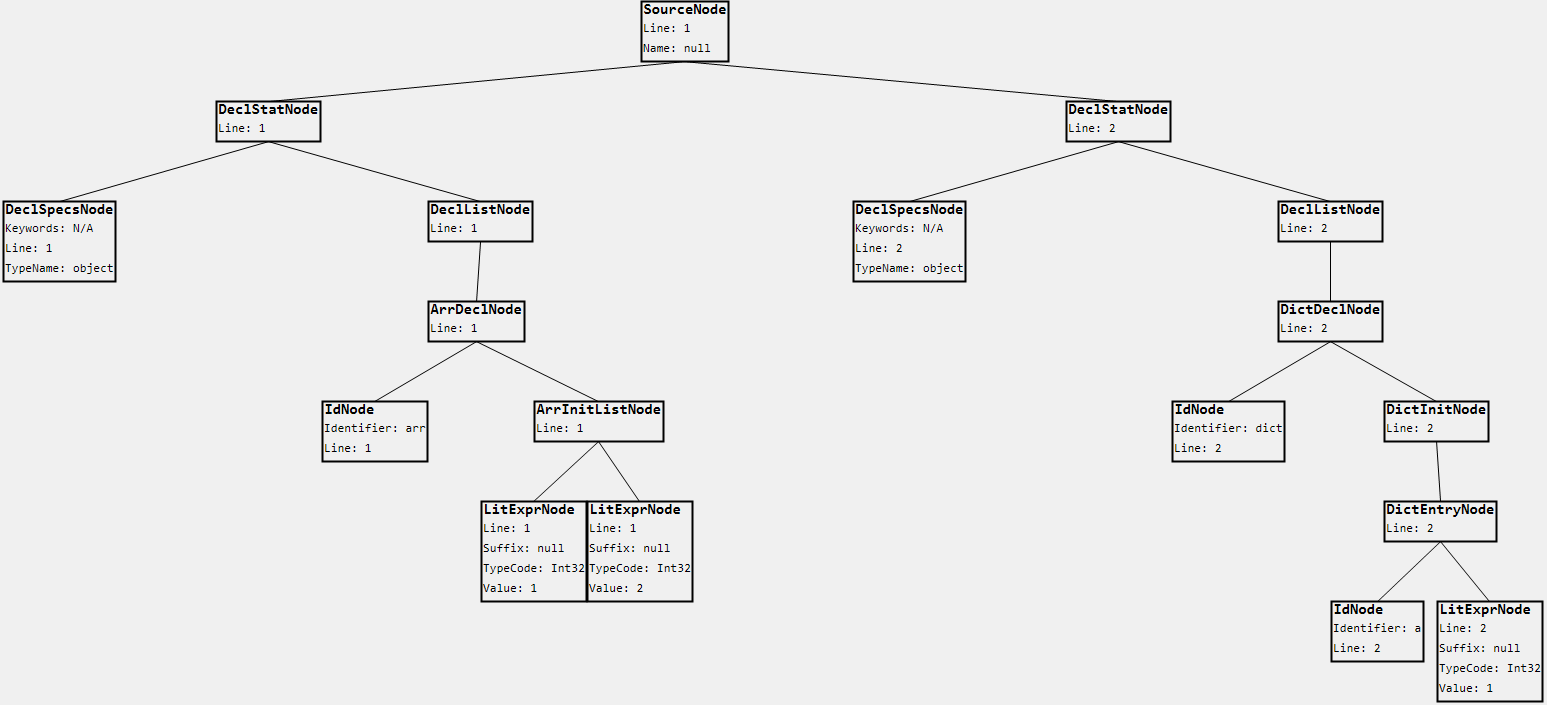
\includegraphics[scale=0.4]{images/lua_ast_decl.png}
\caption{Primer deklaracije promenljive i niza u programskom jeziku Lua i odgovarajući AST.}
\label{fig:MyASTExampleLuaDeclaration}
\end{figure}


\subsection{Čvorovi operatora}
\label{subsec:MyASTOperatorNodes}

Svrha operatora je da vezuju izraze i da tako grade nove izraze. Operator se karakteriše simbolom i \emph{arnošću}, tj. brojem argumenata koje taj operator prima. Na osnovu arnosti, svaki operator se može apstraktno posmatrati kao članica grupe operatora sa istom arnošću. Na slici \ref{fig:OperatorNodes} se može videti hijerarhija operatora korišćena dalje u apstrakciji. Binarni operatori zahtevaju dva operanda i pišu se infiksno, dok unarni zahtevaju jedan operand i pišu se prefiksno. Ternarni operatori koji postoje u nekim programskim jezicima nisu razmatrani jer se mogu posmatrati kao druge strukture\footnote{Na primer, ternarni operator \texttt{?:} prisutan u jezicima zasnovanim na sintaksi programskog jezika C se može zameniti naredbom uslovnog grananja.}. 

\begin{figure}[h!]
\centering
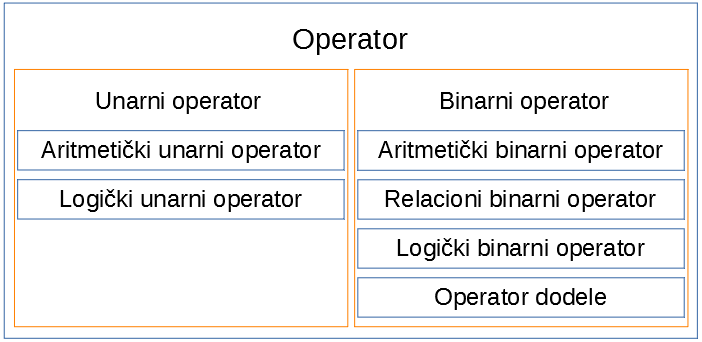
\includegraphics[scale=0.5]{images/operator_nodes.png}
\caption{Podela operatora na osnovu njihove arnosti.}
\label{fig:OperatorNodes}
\end{figure}

Unarni aritmetički operatori su unarni operatori koji figurišu u aritmetičkim izrazima, npr. operator promene znaka, operator bitovske negacije\footnote{Bitovski izrazi se mogu posmatrati kao vrsta aritmetičkih izraza.}, operatori kastovanja ili inkrementiranja odnosno dekrementiranja. Unarni logički operatori su unarni operatori koji figurišu u logičkim izrazima, npr. operator negacije. Možemo sve ove unarne operatore posmatrati apstraktno ukoliko definišemo unarni operator kao strukturu koja definiše unarnu funckiju koja transformiše svoj argument na osnovu logike konkretnog unarnog operatora. Tip argumenta i povratne vrednosti pomenute funkcije zavisi od tipa unarnog operatora --- aritmetički unarni operatori mogu primiti vrednost bilo kog tipa\footnote{Ne postoji ograničenje na brojevne tipove jer se u nekim jezicima operatori mogu predefinisati tako da rade i za korisnički definisane tipove (engl. \emph{operator overloading}).} i vraćaju vrednost proizvoljnog, ne nužno istog tipa; dok unarni logički operatori primaju i vraćaju bulovsku vrednost\footnote{U nekim programskim jezicima postoji implicitna konverzija brojevnih tipova u bulovski tip, što se jednostavno može posmatrati kao poređenje vrednosti po jednakosti sa nulom.}. Koristeći ovaj pristup, nije potrebno praviti novi AST čvor za svaki mogući operator, već je dovoljno da postoji samo jedan čvor koji predstavlja unarni operator. Ovakav pristup odgovara varijanti AST sa regularnošću (videti sliku \ref{fig:ASTVariants}), omogućava opisivanje proizvoljnih operatora i nije vezan za konkretnu programsku paradigmu.

Binarni aritmetički operatori su binarni operatori koji figurišu u aritmetičkim izrazima, npr. operatori koji odgovaraju matematičkim operacijama ali i bitovski binarni operatori. Binarni relacioni operatori su binarni operatori koji figurišu u relacionim izrazima, npr. operatori poretka ($<$, $>$, $\leq$, $\geq$) i poređenja po jednakosti ili različitosti ($=$, $\neq$). Binarni logički operatori su binarni operatori koji figurišu u logičkim izrazima, npr. bulovske operacije ($\wedge$, $\vee$). Slično kao i za unarne operatore, moguće je apstraktno posmatrati sve binarne operatore tako što ih definišemo kao strukturu koja definiše binarnu funkciju koja transformiše argumente na osnovu logike konkretnog binarnog operatora. Tip argumenata i povratne vrednosti te funkcije zavisi od tipa binarnog operatora, kao i u slučaju unarnih operatora --- aritmetički binarni operatori primaju dva argumenta proizvoljnog tipa i vraćaju rezultat proizvoljnog, ne nužno istog tipa; relacioni binarni operatori primaju iste tipove argumenata kao i aritmetički binarni operatori, međutim povratna vrednost mora biti bulovskog tipa; dok logički binarni operatori zahtevaju da argumenti i povratna vrednost budu bulovskog tipa. Pritom, na prvi pogled nije jasno kako se operator dodele može uklopiti u ovaj šablon ali, na osnovu toga da je dodela zapravo sporedni efekat i da se posmatra kao izraz čija je vrednost jednaka vrednosti izraza sa desne strane operatora, može se primeniti isti princip kao i za aritmetičke binarne izraze. Neki programski jezici dozvoljavaju i složene operatore dodele, koji se mogu dekomponovati na više jednostavnijih izraza.

\subsection{Čvorovi izraza}
\label{subsec:MyASTExpressionNodes}

Izraz, kao što se može videti na primeru gramatike sa slike \ref{fig:ANTLRExpressions}, se definiše rekurzivno i izraze mogu proširiti razni operatori. Na slici \ref{fig:ExpressionNodes} se mogu videti tipovi apstraktnih konstrukcija koje će se koristiti da bi se predstavili izrazi. Dodatno, za vezivanje izraza će se koristiti apstrakcije operatora definisane u prethodnom odeljku.

\begin{figure}[h!]
\centering
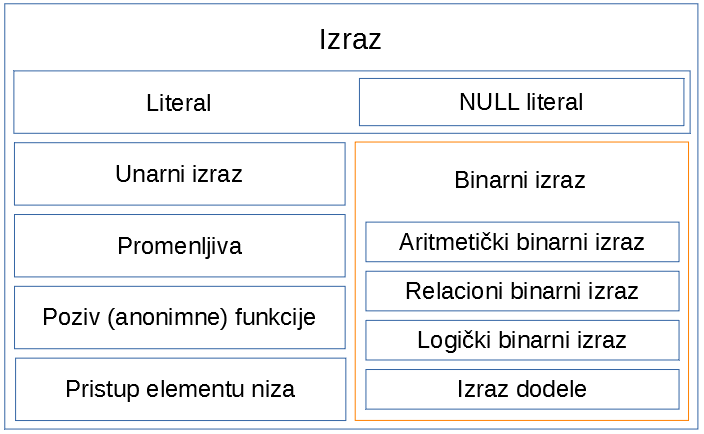
\includegraphics[scale=0.5]{images/expression_nodes.png}
\caption{Vrste čvorova izraza.}
\label{fig:ExpressionNodes}
\end{figure}

Najjednostavniji izraz predstavljaju konstante ili \emph{literali}. Literali mogu biti brojevne konstante, karakterske konstante ili konstantne niske. Literali često mogu imati i sufiks (najčešće za brojevne literale), koji određuje tip literala u slučajevima gde postoji dvosmislenost. Na primer, literal $5$ možemo posmatrati kao 32-bitni ceo broj ili kao 64-bitni ceo broj (ali i kao realan broj, ako ne zahtevamo da realne brojeve moramo pisati u nepokretnom ili pokretnom zarezu). Da bi se ova dvosmislenost uklonila, možemo eksplicitno naznačiti da se govori o 64-bitnom celom broju dodavanjem sufiksa \texttt{L}, ako je u pitanju programski jezik C ili njemu slični jezici. Takođe, pošto nezanemarljiv broj programskih jezika dozvoljava rad sa pokazivačima ili neposredno koristi alokaciju memorije za kreiranje objekata, uobičajeno je korišćenje prazne adrese kao specijalne vrednosti (\texttt{null} ili \texttt{nil}). Za ovu specijalnu vrednost je moguće kreirati poseban tip literala, jer ovaj literal može biti bilo kog tipa koji nije primitivni tip.

Osim literala, samostalne promenljive mogu predstavljati validan izraz, u kom slučaju je vrednost izraza trenutna vrednost te promenljive. Slično važi i za indeksni pristup nizu\footnote{Isto važi i za bilo koju drugu kolekciju, ukoliko je nad njom definisan operator indeksnog pristupa. Predefinisanje ovog operatora nije razmatrano u ovom radu.}. U slučaju indeksnog pristupa, potrebno je navesti izraz čija vrednost označava indeks (to ne mora biti jednostavni literal). Postoje smislena ograničenja šta sve sme da se nađe unutar izraza koji predstavlja indeks elementa niza tako da to semantički ima smisla, ali se na ovom nivou ne bavimo semantičkom analizom. 

Unutar izraza se mogu naći i pozivi funkcija. Naravno, pretpostavljamo da funkcija ima povratnu vrednost, koja će se iskoristiti nakon poziva funkcije u kontekstu iz kojeg je ona pozvana. Pod uticajem funkcionalne paradigme, veliki broj programskih jezika dozvoljava definisanje anonimnih (lambda) funkcija, čija se definicija može smatrati izrazom koji se može dodeliti nekom simbolu. Stoga se i anonimne funkcije mogu smatrati validnim izrazima. 

Operatori opisani u \ref{subsec:MyASTOperatorNodes} mogu vezati sve tipove iznad i formirati složenije izraze. U zavisnosti od broja izraza koje operator vezuje, izraze možemo podeliti na unarne i binarne. Unarne izraze nadograđuju unarni operatori dok su binarni izrazi dobijeni primenom binarnog operatora na dva izraza. U zavisnosti od tipa binarnog operatora (videti sliku \ref{fig:OperatorNodes}), binarne izraze delimo na sličan način. Naravno, svaki od tipova binarnog izraza zahteva odgovarajući tip binarnog operatora. Slično se može uraditi i za unarne izraze, ali takođe i napraviti podela na prefiksne i postfiksne unarne izraze. S obzirom da je cilj napraviti opšti AST, činjenica da li je unarni operator prefiksni ili postfiksni nije od suštinskog značaja, pogotovo ukoliko se uzme u obzir da dva programska jezika mogu imati unarne operatore sa istom semantikom ali različitom pozicijom u odnosu na operand --- u jednom jeziku taj operator može biti prefiksni a u drugom postfiksni. Kako bi poređenje ovakvih operatora funkcionisalo bez obzira na njihovu poziciju u odnosu na operand, u ovom radu nije pravljena podela na prefiksne i postfiksne unarne operatore.

Na slici \ref{fig:MyASTExampleExpressions} se mogu videti kreirani AST za izraz \texttt{(3 + 5) << f(4)}. Ovaj izraz poprima isti oblik bez obzira na to koji je programski jezik u pitanju, ali iako se sintaksa bude razlikovala ili operatori budu imali drugi simbol, logika operatora opisana putem funkcije će ostati ista.

\begin{figure}[h!]
\centering
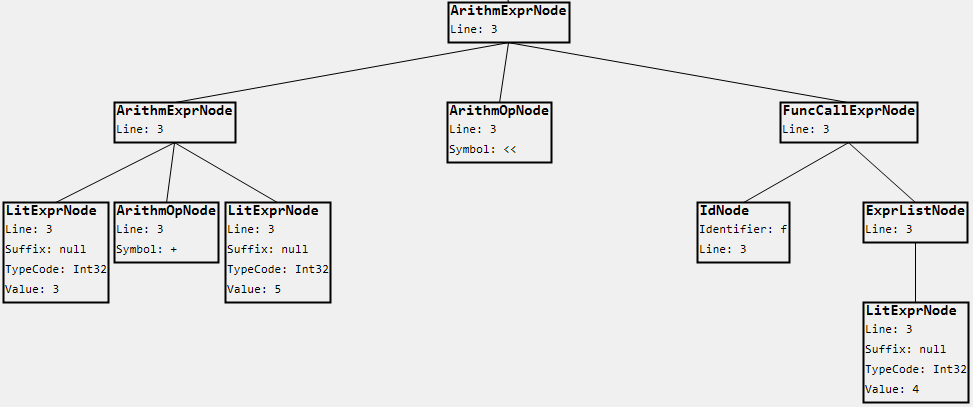
\includegraphics[scale=0.6]{images/ast_expr.png}
\caption{AST generisan od izraza \texttt{(3 + 5) << f(4)}.}
\label{fig:MyASTExampleExpressions}
\end{figure}

\subsection{Čvorovi naredbi}
\label{subsec:MyASTStatementNodes}

Naredbe su najkomplikovanije za apstrahovanje zbog njihove raznovrsnosti. Programski jezici često uvode nove sintaksičke strukture i naredbe koje nisu do tada viđene u ostalim jezicima. Uprkos svemu tome, ipak je moguće uočiti neke sličnosti sa već postojećim konceptima i svesti ih na isti nivo. Na slici \ref{fig:StatementNodes} se mogu videti tipovi apstraktnih konstrukcija koje će se koristiti da bi se predstavile naredbe.

\begin{figure}[h!]
\centering
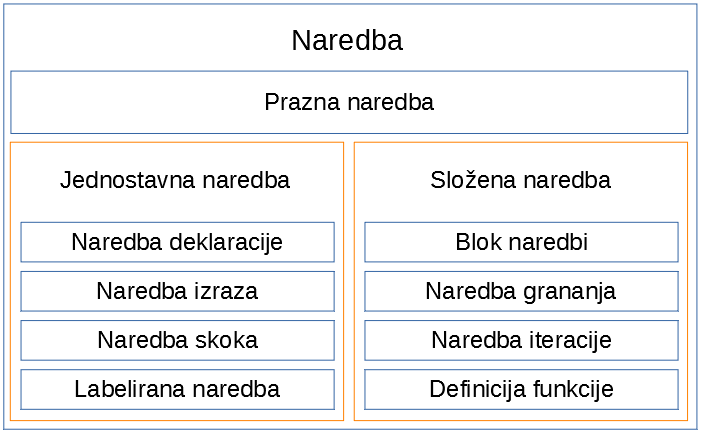
\includegraphics[scale=0.5]{images/statement_nodes.png}
\caption{Vrste čvorova naredbi.}
\label{fig:StatementNodes}
\end{figure}

Veliki broj programskih jezika podržava praznu naredbu, sa semantikom ne izvršavanja nikakvih operacija. U programskim jezicima koji su zasnovani na sintaksi jezika C, praznu naredbu navodimo samo korišćenjem simbola za kraj naredbe (\texttt{;}), dok u programskom jeziku Python koristimo ključnu reč \texttt{pass}. 

Naredbe su podeljene na \emph{jednostavne} i \emph{složene}, koje se sastoje od više drugih naredbi. Primer jednostavne naredbe može biti deklaracija promenljive, dok primer složene naredbe može biti definicija funkcije koja se sastoji od više jednostavnih deklaracija ali možda i drugih složenih naredbi kao što su grananja i petlje.

Jednostavne naredbe uključuju naredbe deklaracije i izraza. Razlog zašto se deklaracije i izrazi opet pojavljuju je taj što izrazi sami po sebi mogu biti deo drugih naredbi. Ukoliko se naredba sastoji samo od izraza, onda nju zovemo naredbom izraza. Primer može biti izraz dodele --- vrednost izraza dodele se može koristiti u drugim izrazima ali, ukoliko samo želimo da izvršimo dodelu i ništa više u okviru iste naredbe, onda izraz dodele "umotavamo" u naredbu izraza. Slično važi i za deklaracije, ukoliko razmotrimo idiomsku \texttt{for} petlju (od standarda C99) --- moguće je deklarisati promenljive koje se koriste unutar ciklusa ali to nije naredba deklaracije već deklaracija koja se koristi unutar druge naredbe. 

Naredbe se mogu označiti, po uzoru na koncept \emph{labele} u imperativnim jezicima --- identifikatorom koji označava lokaciju u izvornom kodu. Labele se u imperativnim jezicima najviše koriste da bi se izvršili skokovi na određene lokacije u kodu ali su takođe prisutne i u proceduralnim jezicima (npr. kroz naredbu višestrukog grananja --- \texttt{switch} ili u nekim jezicima \texttt{case}). Labelirana naredba se sastoji od naredbe i identifikatora koji predstavlja labelu. 

Naredbe skoka se koriste obično u paru sa labeliranim naredbama, ali to ne mora uvek biti slučaj. Iako ove čvorove koristimo da bismo predstavili naredbe skoka prisutne u imperativnim jezicima, one predstavljaju i naredbe prekida (\texttt{break} ili \texttt{continue}) ili povratka vrednosti funkcije (\texttt{return}). U slučaju da je u pitanju skok na određenu labelu, onda se sastoji i od identifikatora koji predstavlja labelu na koju se skače. Ukoliko je u pitanju naredba prekida, nisu potrebne nikakve dodatne informacije (mada se i u tom slučaju može iskoristiti činjenica da su u pitanju skokovi pa se može labelirati petlja na koju se odnosi naredba prekida). U slučaju povratka vrednosti funcije, sadrži opcioni izraz čija vrednost predstavlja povratnu vrednost funkcije.

Složene naredbe se sastoje od više drugih naredbi (ne nužno samo od jednostavnih). Često je potrebno izvršiti više naredbi u okviru jednog konteksta i za to se koristi blok naredba. Blok naredba grupiše više drugih naredbi u jednu. Blok naredba se u proceduralnim jezicima, obično navodi eksplicitno --- recimo za programski jezik C pomoću velikih zagrada (\texttt{\{\}}). Za skript jezike često nije potrebna nikakva eksplicitna oznaka već se blok naredba prepoznaje implicitno ili se navodi korišćenjem različitih nivoa indentacije (Python). Neki skript jezici, na primer Lua, zahtevaju eksplicitno navođenje ključnih reči pre početka i nakon kraja blok naredbe ukoliko je ona deo složenije naredbe.

Naredbe uslovnog grananja se sastoje od \emph{uslova}, koji može biti relacioni ili logički izraz, naredbe koja se vrši ukoliko je uslov ispunjen (\emph{then} grana), i opciono naredbe koja se izvršava ako uslov nije ispunjen (\emph{else} grana). Rezultat uslovnog izraza, iako mora biti istinitosna vrednost, je dozvoljeno da bude bilo kog tipa (dakle nema ograničenja samo na relacione i logičke izraze) iz razloga što određeni programski jezici dozvoljavaju automatsku konverziju brojevnih tipova u logički (C). Štaviše, nekada je moguća i implicitna konverzija određenih tipova u logički tip definisanjem implicitnih operatora konverzije (C\#). Zato će u apstrakciji uslov biti bilo koji izraz. Što se \emph{then} i \emph{else} grana tiče, one mogu biti bilo koje naredbe, ali zarad konzistentnosti će obe biti blokovi naredbi. Na slici \ref{fig:MyASTExampleStatement} se može videti AST za naredbu grananja.

\begin{figure}[h!]
\begin{lstlisting}
do                               something()
    something()                  while (condition) do
while (condition)                    something()
\end{lstlisting}
\begin{lstlisting}
repeat                           something()
    something()                  while (not condition) do
until (condition)                    something()
\end{lstlisting}
\caption{Procedura svođenja ređih tipova petlji (levo) na \emph{while} petlju (desno) prikazana u pseudo-jeziku.}
\label{fig:ASTIterationStatements}
\end{figure}

Naredbe iteracije imaju raznovrsni oblik u programskim jezicima. Najčešće podržane naredbe iteracije su \emph{for} i \texttt{while} petlje. U opštem slučaju, dovoljno je koristiti samo jedan tip petlji, ali zarad jednostavnosti i prisutnosti ovih tipova u velikoj većini programskih jezika oba će biti podržana. Ostali tipovi petlji, kao što su \emph{do-while} ili \emph{repeat-until} petlje, će se svoditi na njih. \emph{do-while} petlja se može svesti na \emph{while} petlju jednostavnim ponavljanjem tela petlje pre same petlje i kreiranjem obične \emph{while} petlje sa istim uslovom i telom. Slično se može uraditi i za \emph{repeat-until} petlju, s tim što je potrebno samo negirati uslov u dobijenoj \emph{while} petlji. Ovaj proces je ilustrovan na slici \ref{fig:ASTIterationStatements}. 

\begin{figure}[h!]
\centering
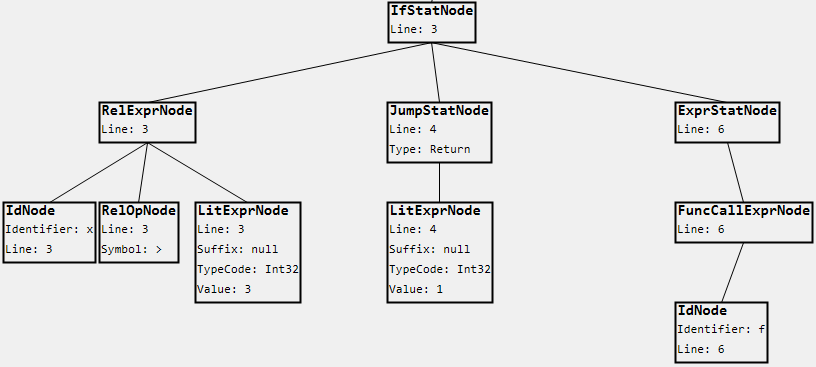
\includegraphics[scale=0.7]{images/ast_stat.png}
\caption{AST naredbe grananja.}
\label{fig:MyASTExampleStatement}
\end{figure}



\chapter{Semantičko poređenje opštih AST}
\label{chp:ASTComparing}

Jedna od motivacija svođenja imperativnih jezika na isti nivo apstrakcije može biti poređenje kodova pisanih u različitim programskim jezicima. Pritom, s obzirom da su u pitanju stabla, moguće je koristiti razne algoritme za poređenje stabala (ali i grafova uopšte) nad ovakvim apstrakcijama. Dodatno, potrebno je i definisati kriterijum poređenja --- moguće je porediti kodove \emph{strukturno}, \emph{semantički} itd. U ovom radu je od značaja semantička ekvivalentnost, koja je u opštem slučaju neodlučiv problem. Međutim, ukoliko se ograničimo samo na strukturno slične kodove, moguće je dobiti smislene rezultate u praksi, nalik na one dobijene u ovom radu. Precizna definicija strukturne sličnosti se obično iskazuje u terminima sličnosti strukture njihovih apstrakcija. Naravno, postoje kodovi koji nisu strukturno ekvivalentni ali su semantički ekvivalentni --- takvi slučajevi se onda neće razmatrati zbog neispunjenosti pretpostavke o strukturnoj sličnosti. 

Pretpostavka strukturne sličnosti je ograničavajuća i znatno smanjuje broj slučajeva upotrebe takvog upoređivača. Međutim, danas je od velikog značaja provera ispravnosti programa dobijenih sitnim refaktorisanjem već postojećih programa, nekada ne menjajući strukturu uopšte (a ako se struktura koda menja onda se to obično radi u manjim koracima između kojih i dalje može da važi pretpostavka strukturne sličnosti kodova u susednim koracima). Slično, prepisivanje programa sa jednog programskog jezika na drugi se javlja najčešće prilikom migracija na nove tehnologije. U takvim situacijama implicitno je prisutna strukturna slučnost, što zavisi od konkretnih programskih jezika ali se u praksi često smanjuje napor tako što se održava struktura koda, barem u inicijalnim verzijama. 

Definicija strukturne sličnosti za potrebe ovog rada će se odnositi na sličnosti u rasporedu blokova naredbi dok će raspored naredbi u blokovima biti nebitan. Na primer, ukoliko se prvi program sastoji od bloka naredbi u kome se nalaze dva druga bloka, očekuje se da i drugi program ima istu organizaciju blokova, pri čemu se pod terminom blok podrazumevaju i složene naredbe koje se sastoje od bloka naredbi u sebi, kao što su definicije funkcija, uslovna grananja, petlje i ostali tipovi složenih naredbi opisanih u \ref{subsec:MyASTStatementNodes}. Pod ovim uslovima, moguće je porediti blokove prvog programa sa odgovarajućim blokovima drugog programa.

Neophodno je napomenuti da se apstahovanjem gube informacije koje su od važnosti za statičku analizu, stoga sve pozitivne rezultate analize sprovedene u ovom radu je potrebno pažljivo razmotriti. Konkretno, tipovi podataka u jezicima koji ne propisuju striktno veličinu tipova (npr.~celobrojni tip u programskom jeziku C) možda neće biti pravilno predstavljeni u apstrakciji. Prilikom rada sa ovim vrednostima u nekim slučajevima može doći do prekoračenja, ili nedostatka prekoračenja, što je različito ponašanje od originalnog. Takođe, ukoliko se apstrahuje specifikacija pisana u programskom jeziku koji ne propisuje striktno redosled izračunavanja operanada izraza, prilikom analize neće nužno biti isti redosled izvršavanja operanada izraza u odnosu na specifikaciju.

\section{Simboličko izračunavanje}
\label{sec:Symbolics}

Današnji softver je veoma kompleksan i često funkcioniše na različitim nivoima arhitekture velikih projekata. Stoga je proces verifikacije softvera veoma značajan i delikatan. U procesu verifikacije se najčešće koriste ručno pisani testovi i pregledi koda od strane drugih programera. Uprkos svim ovim merama, greške su i dalje nezaobilazne --- jedan test može proveriti ponašanje koda za samo jedan ulaz. S obzirom da je nemoguće testirati sve ulaze zbog njihovog ogromnog broja (ukoliko posmatramo samo funkciju jedne promenljive koja prima 32-bitni ceo broj, broj mogućih ulaza je $2^{32}$) potrebno je da testovi dobro \emph{generalizuju} --- da pokrivaju opšte ali i neke specijalne ulaze. To se postiže uočavanjem da se vrednosti ulaza mogu razvrstati u klase po tome kakav izlaz uzrokuju. Ukoliko imamo funkciju koja deli dva broja, te klase mogu biti celi brojevi, realni brojevi, neke specijalne vrednosti specifične za operaciju deljenja (recimo $0$), kao i granice za tip podataka iz čijeg domena argumenti funkcije mogu uzeti vrednost. Čak i ovakav pristup, iako drastično smanjuje broj testova i eliminiše redundantne testove, i dalje zahteva relativno veliki broj testova u slučaju većih projekata i stoga je teško pronaći sve greške, pogotovo u slučajevima koji se retko dešavaju i ako ispoljavanje istih zavisi od stanja drugih komponenti ili pak nekih nedeterminističkih ponašanja samog sistema. Poželjno je čitav izvorni k\^od pokriti  testovima (engl. \emph{code coverage}) --- iako dostignuta pokrivenost koda od 100\% i dalje ne znači da taj k\^od ispravno radi.

\emph{Statička analiza koda} predstavlja analizu izvornog koda bez pokretanja istog sa ciljem ispitivanja stanja u kojima se može naći program i proveru rada jedinice koja se testira za mnogobrojne ulaze. Iako ispravna u teoriji, u praksi nailazi na puno problema --- osnovni je razlika u apstrakcijama koju prave statički analizator i programer.

\emph{Simboličko izvršavanje} \cite{SymbolicExecution} predstavlja sredinu između klasične verifikacije putem pisanja testova i statičke analize koda. Prilikom simboličkog izvršavanja, umesto stvarnih vrednosti ulaza koriste se \emph{simboličke promenljive}. Simbolička promenljiva nije vezana za specifičnu vrednost i analiza se dalje vrši samo nad njom --- samim tim se istovremeno mogu testirati višestruke klase sličnih ulaza. 

Primer simboličkog izvršavanja će biti opisan na isečku C koda sa slike \ref{fig:SymbolicExecCode}. Pretpostavimo da imamo deklarisanje promenljive \texttt{a}, \texttt{b} i \texttt{c} i da se neke operacije izvršavaju nad njima, reprezentovano komentarom u liniji $3$. U nekom trenutku se vrednosti tih promenljivih koriste kao uslovi od kojih zavisi prolaznost testa u poslednjoj liniji. Dodelimo svakoj promenljivoj simboličku vrednost --- \texttt{a = }$\alpha$, \texttt{b = }$\beta$, \texttt{c = }$\gamma$. Možemo izgraditi stablo izvršavanja i uslove koji moraju da važe nad simboličkim vrednostima $\alpha$, $\beta$ i $\gamma$ kako bi test u poslednjoj liniji prošao.

\begin{figure}[h!]
\begin{lstlisting}[language={}]
int a, b, c;

// ...

int x = 0, y = 0, z = 0;
if (a)      
    x = -2;
if (b < 5)  {
    if (!a && c)    
        y = 1;
    z = 2;
}

assert(x + y + z != 3);
\end{lstlisting}
\caption{Isečak C koda dat kao primer nad kojim će se prikazati simboličko izvršavanje.}
\label{fig:SymbolicExecCode}
\end{figure}

Ukoliko put izvršavanja programa zavisi od simboličke promenljive, kao što je to slučaj za izvorni k\^od sa slike \ref{fig:SymbolicExecCode}, simbolička promenljiva se konceptualno "grana" i analiza se nastavlja za oba slučaja posebno. Tako se dobija drvo izvršavanja, gde svaka putanja odgovara mnogim individualnim testovima koji bi uzrokovali prolazak izvršavanja tom putanjom. Vrednosti promenljivih u tim testovima moraju zadovoljiti uslove na kraju svake putanje --- tzv. \emph{uslove putanje} (engl. \emph{path conditions}). Odgovarajuće stablo izvršavanja za izvorni k\^od sa slike \ref{fig:SymbolicExecCode} sa definisanim simboličkim vrednostima $\alpha$, $\beta$ i $\gamma$ se može videti na slici \ref{fig:SymbolicExecTree}. Svaka naredba dodele je uokvirena pravougaonikom dok je uslov uokviren elipsom. Boje grana odgovaraju istinitosnoj vrednosti uslova iz poslednje linije u tom trenutku. Na kraju svake grane se nalazi uslov putanje za tu granu koje u nekim slučajevima može jedinstveno odrediti vrednost simboličke promenljive koja dovodi do prolaska tom putanjom ili u opštem slučaju generisati test primer koji dovodi do prolaska tom putanjom. Dakle, ukoliko je stablo simboličkog izvršavanja poznato, moguće je generisati kontra-primere koji pokazuju da program ne radi kao što je očekivano.

\begin{figure}[h!]
\centering
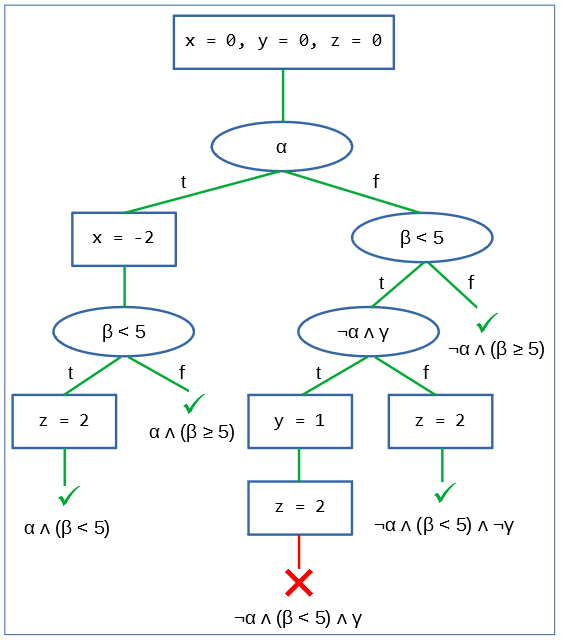
\includegraphics[scale=0.7]{images/sym_tree.png}
\caption{Drvo simboličkog izvršavanja na kom su prikazane sve putanje koje se razmatraju. Na kraju svake grane je napisan uslov koji mora da važi da bi se došlo do lista te grane.}
\label{fig:SymbolicExecTree}
\end{figure}

Simboličko izvršavanje, iako konceptualno moćno, ima par problema koji su uzrokovani pre svega kompleksnošću problema koji se rešava:
\begin{itemize}
    \item \emph{Eksplozija putanja} --- Broj putanja izvršavanja eksponencijalno zavisi od broja uslovnih grananja u kodu. Ukoliko imamo tri naredbe grananja, broj putanja izvršavanja je $2^3=8$. Štaviše, dovode do značajnog uvećanja broja stanja, jer ukoliko u petlji postoji uslov koji zavisi od simboličke vrednosti koja uzima vrednosti iz opsega 32-bitnog celog broja, broj putanja kroz petlju je u tom slučaju $2^{31}$, a u nekim slučajevima i beskonačan. Slično važi i za rekurziju.
    \item \emph{Ograničenja rešavača} --- Kako broj putanja raste, povećava se i broj uslova koji se moraju zadovoljiti prilikom nalaženja kontraprimera. U nekim slučajevima je moguće osloniti se na \emph{SMT rešavače} \cite{SMT} za nalaženje kontra-primera kako bi se ublažio ovaj problem.
    \item \emph{Modelovanje podataka} (engl. \emph{heap modelling}) --- Kreiranje simboličkih struktura podataka i pokazivača nije jednostavan proces.
    \item \emph{Modelovanje okruženja} (engl. \emph{environment modelling}) --- Nije uvek jednostavno adaptirati mehanizam za česte potrebe prilikom dizajna softvera kao što je korišćenje eksternih biblioteka i sistemskih poziva ali i specifičnosti sistema.
\end{itemize}

Postoji dosta alata i biblioteka koje pružaju interfejs za simboličko izračunavanje u raznim programskim jezicima --- jedan od najpoznatijih alata za simboličko izračunavanje je \emph{KLEE} \cite{KLEE}, izgrađen nad \emph{LLVM} infrastruktorom \cite{LLVM} \cite{LLVM04} i dizajniran za analizu koda pisanog u programskom jeziku C. U ovom radu je simboličko izvršavanje korišćeno za detekciju razlika u vrednostima promenljivih uz pomoć biblioteka za programski jezik C\#.

\section{Algoritam za semantičko poređenje}
\label{sec:ASTComparingAlgorithm}

U ovom radu je poređenje vršeno pomoću algoritma pisanog specifično za rad sa opštim apstrakcijama opisanim u \ref{sec:MyAST}. Grubi opis algoritma za poređenje, u daljem tekstu \emph{upoređivač}, je prikazan na slici \ref{fig:ComparisonAlgorithmPseudo}. Upoređivač se sastoji od više upoređivača koje porede specifične tipove čvorova. Za početak, potreban je jedan adapter koji će dobiti pokazivače na korene stabala koje je potrebno uporediti. S obzirom da tipovi čvorova mogu biti različiti, potrebno je proveriti da li su tipovi isti. Ukoliko to nije slučaj, prijavljuje se greška i rad se prekida. U protivnom, potrebno je odrediti tip čvorova i pozvati konkretni algoritam za poređenje. 

\begin{figure}[!h]
\begin{algorithmic}[1]
\Procedure{Uporedi}{$n_1$, $n_2$}
\If{\emph{$n_1$ i $n_2$ su istog tipa}}
    \State $t \gets$ \emph{tip čvora $n_1$}
    \If{\emph{postoji definisan upoređivač za čvorove tipa} $t$}
        \State $U \gets$ \emph{upoređivač čvorova tipa $t$}
        \State \textbf{return} U$(n_1, n_2)$
    \Else
        \If{$\text{BrojDece}(n_1) \neq \text{BrojDece}(n_2)$}d
            \State \textbf{return} \texttt{False}
        \Else        
            \If{$\text{Atributi}(n_1) \neq \text{Atributi}(n_2)$}
                \State \textbf{return} \texttt{False}
            \EndIf
            \For{$i \gets 0$ \textbf{to} $\text{BrojDece}(n_1)$}
                \State $d_1 \gets $ \emph{dete $i$ čvora $n_1$}
                \State $d_2 \gets $ \emph{dete $i$ čvora $n_2$}
                \If{\textbf{not} $\text{Uporedi}(d_1, d_2)$}
                    \State \textbf{return} \texttt{False}
                \EndIf
            \EndFor
            \State \textbf{return} \texttt{True}
        \EndIf
    \EndIf
\Else
    \State \textbf{return} \texttt{False}
\EndIf
\EndProcedure
\end{algorithmic}
\caption{Osnovni AST upoređivač.}
\label{fig:ComparisonAlgorithmPseudo}
\end{figure}

Podrazumevana implementacija poređenja može biti takva da se uporede atributi svih čvorova a zatim se svako dete prvog čvora rekurzivno uporedi sa odgovarajućim detetom drugog čvora (ukoliko imaju isti broj dece). Ako neki par dece nije ekvivalentan, onda to ne važi ni za njihove roditelje. Za većinu tipova čvorova ovakvo poređenje je dovoljno. 

Naredbe koje se sastoje od više drugih naredbi, kao što su npr.~definicije funkcija ili petlje, se moraju porediti drugačije jer složena naredba može sadržati lokalne promenljive. Niz naredbi koji predstavlja jednu složenu naredbu će u nastavku biti referisan pod terminom \emph{blok} ili \emph{blok naredbi}. Za poređenje blokova naredbi je stoga definisana posebna procedura poređenja opisana u nastavku.


\section{Upoređivač blokova naredbi}
\label{sec:ASTComparingBlocks}

Podrazumevani način poređenja dece svakog čvora nije dobar u opštem slučaju za blokove naredbi jer je osetljiv na izmene redosleda naredbi --- na primer promena redosleda deklaracija. Stoga je upoređivač blokova potrebno napisati tako da može da uoči semantičku ekvivalentnost iako naredbe nisu nužno jednake, a možda ih čak ima i različit broj.

Upoređivač se zasniva na poređenju vrednosti promenljivih na kraju svakog bloka naredbi. Apstrakcije dva programa se porede paralelno --- \emph{blok-po-blok}. Naredbe svakog bloka se izvršavaju i prate se izmene vrednosti promenljivih deklarisanih do tog trenutka (bilo u bloku koji se trenutno razmatra, ili u roditeljskim blokovima). Na kraju svakog bloka se vrši provera jednakosti simboličkih vrednosti promenljivih iz oba programa deklarisanih do tog trenutka i svaka razlika se prijavljuje kao potencijalna greška. Pošto broj promenljivih u programima ne mora biti isti iako su oni semantički ekvivalentni, za one promenljive koje nemaju parnjaka prilikom poređenja se prijavljuju upozorenja ali ne i greške ukoliko nije bilo konflikata prilikom poređenja vrednosti ostalih promenljivih. Upoređivač blokova naredbi je prikazan na slici \ref{fig:ComparisonAlgorithmBlocksPseudo}.

\begin{figure}[!h]
\begin{algorithmic}[1]
\Procedure{UporediBlokove}{$b_1$, $b_2$}
\State $gds_1 \gets $ \emph{simboli iz svih predaka bloka $b_1$}
\State $gds_2 \gets $ \emph{simboli iz svih predaka bloka $b_2$}
\State $lds_1 \gets $ \emph{lokalni simboli za blok $b_1$}
\State $lds_2 \gets $ \emph{lokalni simboli za blok $b_2$}
\State $\text{UporediSimbole}(lds_1, lds_2)$
\State $\text{IzvrsiNaredbe}(b_1, b_2, lds_1, lds_2, gds_1, gds_2)$
\State \textbf{return} $\text{UporediSimbole}(lds_1, lds_2) \wedge \text{UporediSimbole}(gds_1, gds_2)$
\EndProcedure
\end{algorithmic}
\caption{Upoređivač blokova naredbi.}
\label{fig:ComparisonAlgorithmBlocksPseudo}
\end{figure}

U opisu algoritma se koristi termin \emph{simbol} koji se sastoji od identifikatora i simboličke vrednosti promenljive. Lokalni simboli su deklarisani unutar bloka dok su globalni simboli deklarisani van trenutnog bloka a mogu se referisati iz njega. Pronalaženje deklarisanih simbola u bloku podrazumeva prolaz kroz naredbe bloka i registrovanje svih naredbi deklaracije, izvlačenje deklaratora iz njih i, uzimajući u obzir opcione inicijalizatore, kreiranje simboličke vrednosti za upravo deklarisani identifikator. Identifikator i opcioni simbolički inicijalizator čine \emph{simbol}. Isto se ponavlja za sve naredbe deklaracije u bloku i rezultat je skup deklarisanih simbola.

Nakon registrovanja svih lokalnih simbola proverava se njihova ekvivalentnost u funkciji \texttt{UporediSimbole}. Ova funkcija proverava da li se svi simboli iz prvog bloka nalaze u drugom i prijavljuje ukoliko neki simboli fale ili ukoliko postoje simboli koji su višak. Zatim, za simbole koji se nalaze u oba skupa, proverava njihove simboličke vrednosti. Ukoliko su te vrednosti različite, prijavljuje se potencijalna greška i na osnovu toga da li je bilo konflikata vraća se istinitosna vrednost. Razlog zašto se ta vrednost ne koristi dalje nakon prvog poziva ove funkcije je ta što različiti inicijalizatori ne znače nužno da postoji problem. Problem postoji ukoliko se nakon izvršavanja svih naredbi i dalje dešavaju konflikti u simboličkim vrednostima za neke promenljive. 

Procedura \texttt{IzvrsiNaredbe} izvršava paralelno naredbe iz oba bloka i na osnovu toga koje su naredbe u pitanju može i da ažurira simboličke vrednosti unutar skupova deklarisanih simbola. Pseudokod ove procedure je dat na slici \ref{fig:ComparisonAlgorithmBlocksPseudo1}. Naredbe se za svaki blok izvršavaju dok se ne naiđe do naredbe iz koje se može izvući novi blok --- to mogu biti naredbe grananja, iteracije, definicije funkcija i slično. Sve naredbe do pronađene naredbe se izvršavaju. Procedura \texttt{IzvrsiNaredbu} će proveriti tip naredbe i, u zavisnosti od toga da li je to naredba dodele, eventualno promeniti vrednosti u skupovima prosleđenih simbola. Nakon izvršavanja svih naredbi do pronađene naredbe koja sadrži blok, izvlači se blok iz nje (to isto se radi i za drugi program). Kad se blokovi izvuku, rekurzivno se poziva upoređivač blokova za pronađene parnjake. Po povratku iz rekurzivnog poziva nastavlja se isti postupak sve dok se ne izvrše sve naredbe. Pritom, algoritam se oslanja na strukturnu sličnost --- ukoliko jedan AST ima više blokova na istoj dubini u odnosu na drugi, poređenje možda neće uočiti neke razlike jer neki blokovi neće imati svog parnjaka ili njihovo uparivanje nije jednoznačno. 

Takođe je važno napomenuti da procedura \texttt{IzvrsiNaredbe} vraća povratnu vrednost koja se u algoritmu sa slike \ref{fig:ComparisonAlgorithmBlocksPseudo} ignoriše. Razlog za to je što, u nekim slučajevima, iako su unutrašnji blokovi naredbi različiti, želimo ipak da proverimo vrednosti promenljivih pre nego što zaključimo da postoji problem. Ukoliko, doduše, samo poredimo par čvorova složenih naredbi koje se sastoje od više jednostavnijih naredbi, u tom slučaju ćemo iskoristiti povratnu vrednost ove procedure jer ne postoji širi kontekst iz kojeg pozivamo ovu proceduru.

\begin{figure}[!h]
\begin{algorithmic}[1]
\Procedure{IzvrsiNaredbe}{$b_1$, $b_2, lds_1, lds_2, gds_1, gds_2$}
\State $n_1 \gets $ \emph{niz naredbi bloka $b_1$} 
\State $n_2 \gets $ \emph{niz naredbi bloka $b_2$}
\State $i \gets j \gets 0$
\State $ni \gets nj \gets 0$
\State $eq \gets $ \texttt{True}
\While{\texttt{True}}
    \State $ni \gets $ \emph{indeks prve naredbe koja sadrži blok u $n_1$ počev od indeksa $ni$}
    \State $nj \gets $ \emph{indeks prve naredbe koja sadrži blok u $n_2$ počev od indeksa $nj$}
    \For{$naredba \in \{n_1[x] \mid x \in [i..ni]\}$}
        \State $\text{IzvrsiNaredbu}(naredba, lds_1, gds_1)$
    \EndFor
    \State $i \gets i + ni$
    \For{$naredba \in \{n_2[x] \mid x \in [j..nj]\}$}
        \State $\text{IzvrsiNaredbu}(naredba, lds_2, gds_2)$
    \EndFor
    \State $j \gets j + nj$
    \If{$i > \text{Duzina}(n_1) \vee j > \text{Duzina}(n_2)$}
        \State \textbf{prekini petlju}
    \EndIf
    \State $nb_1 \gets $ \emph{izvuci blok iz naredbe $n_1[i]$}
    \State $nb_2 \gets $ \emph{izvuci blok iz naredbe $n_2[j]$}
    \State $eq \gets eq \wedge \text{UporediBlokove}(nb_1, nb_2)$
    \State $i \gets i + 1$
    \State $j \gets j + 1$
\EndWhile
\State \textbf{return} $eq$
\EndProcedure
\end{algorithmic}
\caption{Upoređivač blokova naredbi.}
\label{fig:ComparisonAlgorithmBlocksPseudo1}
\end{figure}


\chapter{Implementacija}
\label{chp:Implementation}

U ovom poglavlju će biti opisana implementacija pratećeg projekta nazvanog \emph{Language Invariant Code Comparer} (skr. \emph{LICC}), pisanog u programskom jeziku C\# 8.0, koristeći \emph{.NET Core 3.1} radni okvir. C\# je izabran zbog lakoće implementacije velikih projekata i velike podrške paketa koji se mogu preuzeti, od kojih su korišćeni \emph{ANTLR Runtime} paket koji daje potrebne biblioteke za rad sa ANTLR generisanim parserima i \emph{Math.NET Symbolics} paket za rad sa simboličkim vrednostima. Rezultat je konzolna aplikacija koja može da generiše, serijalizuje ili prikaže opšti AST za dati izvorni k\^od, ali i da poredi takav AST sa drugim. Čitav projekat je dostupan u potpunosti na servisu GitHub na adresi \url{https://github.com/ivan-ristovic/LICC}.

Jedan od glavnih ciljeva aplikacije je modularnost i jednostavna proširivost. U tom duhu se, pored implementacije klasa potrebnih za predstavljanje opšte AST apstrakcije, pruža i interfejs za kreiranje adaptera koji će od proizvoljnog stabla parsiranja kreirati opšti AST. Kao primer, adapteri su kreirani za programske jezike C i Lua, a za primer potpune slobode u izboru gramatike je kreirana gramatika za pseudo-jezik i adapter za istu, što dozvoljava poređenje kodova sa specifikacijom datom u obliku pseudo-koda. Čitav projekat se sastoji od više komponenti, organizovanih po prostorima imena, od kojih su značajnije:
\begin{itemize}
    \item \texttt{LICC} --- Glavni program (korisnički interfejs) koji omogućava generisanje, prikaz, serijalizaciju i poređenje AST.
    \item \texttt{LICC.AST} ---Biblioteka klasa za rad sa opštom AST apstrakcijom.
    \item \texttt{LICC.Core} --- Upoređivač opštih AST --- konzolni izlaz.
    \item \texttt{LICC.Visualizer} --- Komponenta za vizualizaciju --- grafički prikaz AST.
    \item \texttt{LICC.Tests} --- Prateći testovi jedinica koda i integracioni testovi.
\end{itemize}

Čitava arhitektura data putem UML dijagrama komponenti se može videti na slici \ref{fig:ImplementationComponents}. Osim implementacije same aplikacije, svaki funkcionalni deo projekta prate i testovi jedinica koda, koji su povezani sa \emph{GitHub Actions} porškom za neprekidnu integraciju (engl. \emph{continuous integration}, srk. \emph{CI}). CI omogućava prevođenje izvornog koda nakon svake izmene kao i izvršavanje akcija nakon prevođenja kao što su testiranje ili generisanje predmeta za upotrebu (engl. \emph{artifacts}) koji predstavljaju rezultat procesa prevođenja i mogu se direktno isporučiti.

\begin{figure}[h!]
\centering
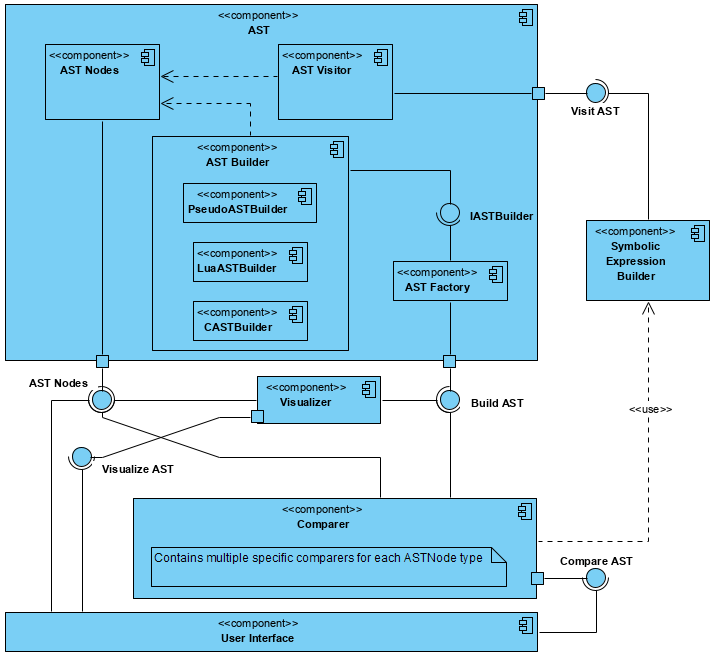
\includegraphics[scale=0.8]{images/uml/ComponentDiagram.png}
\caption{UML dijagram komponenti implementacije.}
\label{fig:ImplementationComponents}
\end{figure}


\section{Implementacija apstrakcije}
\label{sec:ImplementationMyAST}

Implementacija prati hijerarhije opisane u poglavlju \ref{chp:MyAST} kroz mehanizam nasleđivanja. Svaki tip čvora je implementiran kao zasebna klasa koja nasleđuje apstraktnu klasu \texttt{ASTNode}. Dijagram klasa koje nasleđuju klasu \texttt{ASTNode} se može videti na slikama \ref{fig:UMLASTNode1} i \ref{fig:UMLASTNode2}. Pored implementacije klasa koje predstavljaju AST čvorove, kreiran je i javno dostupni interfejs za obilazak AST putem obrazca posetilac u implementaciji korišćen za kreiranja graditelja simboličkog izraza od AST koji predstavlja izraz kao i evaluatora takvog AST.

\begin{figure}[h!]
\centering
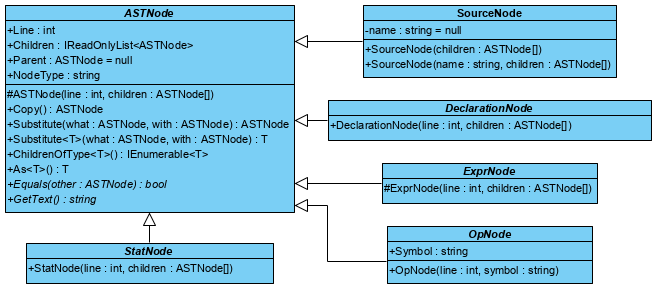
\includegraphics[scale=0.7]{images/uml/ASTNode.png}
\line(1,0){450}\\
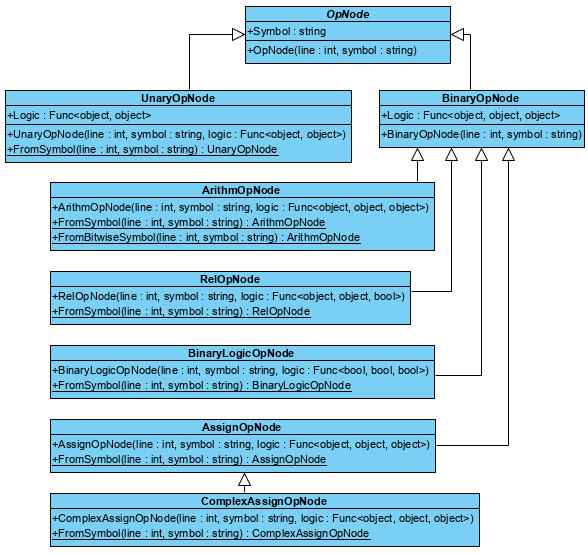
\includegraphics[scale=0.7]{images/uml/OperatorNode.png}
\caption{UML klasni dijagram (deo 1).}
\label{fig:UMLASTNode1}
\end{figure}

\begin{figure}[h!]
\centering
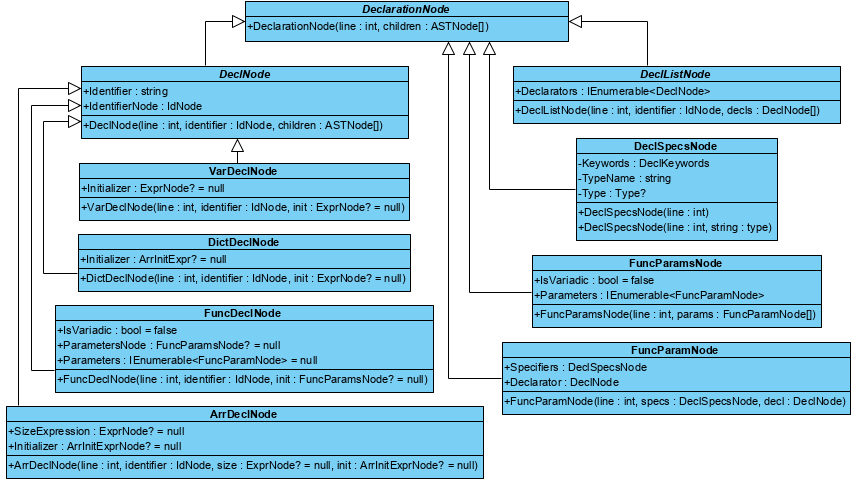
\includegraphics[scale=0.65]{images/uml/DeclarationNode.png}
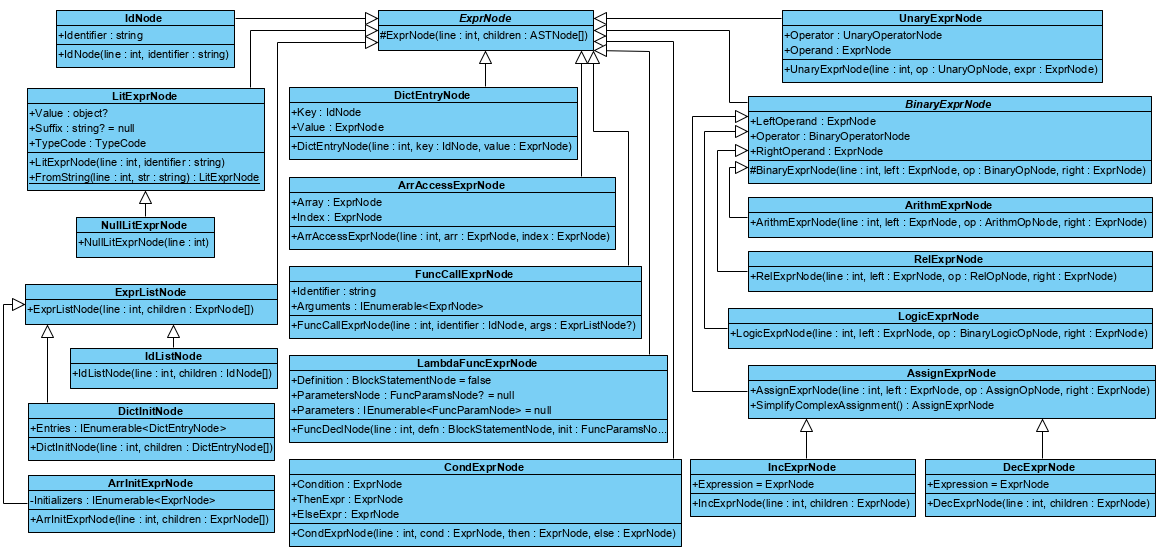
\includegraphics[scale=0.55]{images/uml/ExpressionNode.png}
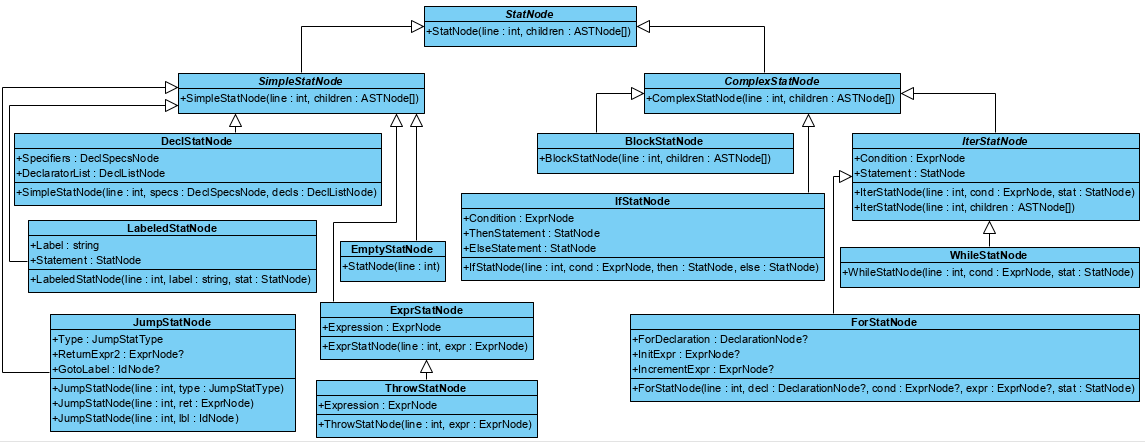
\includegraphics[scale=0.55]{images/uml/StatementNode.png}
\caption{UML klasni dijagram (deo 2).}
\label{fig:UMLASTNode2}
\end{figure}

AST struktura je \emph{imutabilna} --- ne mogu se dodavati ili uklanjati deca čvorovima. Moguće je klonirati AST čvorove ili vršiti zamenu određenog podstabla drugim podstablom ne menjajući original. Svaki AST čvor se može porediti po jednakosti sa drugim AST čvorom po intuitivnoj logici poređenja pruženom kroz predefinisane operatore poređenja.

\section{Implementacija upoređivača}
\label{sec:ImplementationComparer}

Implementacija algoritma upoređivača opisana u poglavlju \ref{chp:ASTComparing} se svodi na implementaciju funkcija za poređenje za svaki tip AST čvora. Te funkcije su enkapsulirane u klase koje implementiraju interfejs za upoređivač čvorova. Te klase nisu javne, tako da se poređenje vrši kroz upoređivač koji poredi instance tipa \texttt{ASTNode}, a koji putem refleksije određuje konkretni tip čvorova i, ukoliko su tipovi isti, pronalazi konkretni upoređivač i poziva operaciju interfejsa upoređivača. Upoređivači međusobno pozivaju jedni druge, kako bi se logika poređenja uprostila --- pošto se naredbe deklaracije sastoje od specifikatora deklaracije i liste deklaratora, upoređivač naredbi deklaracije može pozivati upoređivač za specifikatore deklaracije i upoređivač za listu deklaratora. 

Upoređivač kao rezultat svog rada vraća kolekciju potencijalnih problema (upozorenja ili grešaka) koje je detektovao prilikom analize. Ovakav pristup je odabran zbog lakoće testiranja upoređivača, s obzirom da se može očekivati određena kolekcija problema za određeni izvorni kod. Problem se modeluje kao apstraktna klasa \texttt{BaseIssue} dok se upozorenja ili greške modeluju kroz njene konkretizacije \texttt{BaseWarning} i \texttt{BaseError}. Konkretne greške, kao što su npr. nedostatak deklaracija se mogu onda modelovati kao konkretizacije ovih klasa u zavisnosti od ozbiljnosti problema. Primer izlaza upoređivača za algoritam \emph{swap} se može videti na slici \ref{fig:ComparerSwap}.

\begin{figure}[h!]
\centering
%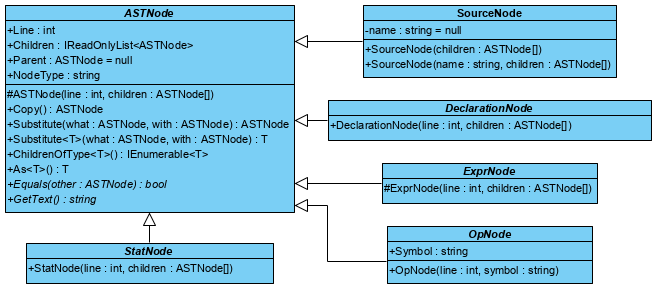
\includegraphics[scale=0.7]{images/uml/ASTNode.png}
\caption{Rezultat rada upoređivača za \texttt{swap} algoritam.}
\label{fig:ComparerSwap}
\end{figure}

\section{Implementacija vizualnog prikaza AST}
\label{sec:ImplementationVisualizer}

Osim serijalizacije AST u JSON format, kreiran je potprogram za vizualni prikaz AST-a (u daljem tekstu \emph{vizualizator}). Primeri izlaza vizualizatora se mogu videti na slikama iz poglavlja \ref{chp:MyAST} --- \ref{fig:MyASTExampleCDeclaration}, \ref{fig:MyASTExampleLuaDeclaration}, \ref{fig:MyASTExampleExpressions} i \ref{fig:MyASTExampleStatement}. Prikaz je izvršen koristeći nativni \texttt{Graphics} paket i, s obzirom da je u pitanju \emph{.NET Core 3.1} radni okvir, moguće je dobiti vizualni prikaz nezavisno od sistema.

Vizualizacija počiva na rekurzivnom algoritmu prikaza u dubinu --- za svaki čvor se prikažu potomci, rasporede jednako po širini, a onda se roditelj centrira u odnosu na ukupnu širinu koju zauzimaju deca. Ovaj pristup nije prostorno optimalan, zbog varijacija u broju dece za čvorove različitih tipova. Što se informacija za svaki čvor tiče, prikazuju se vrednosti svih atributa čvora zajedno sa njegovim tipom u zaglavlju kao i grane do njegovih potomaka.

\section{Implementacija korisničkog interfejsa}
\label{sec:ImplementationUI}

S obzirom da je aplikacija konzolna (osim komponente za vizualizaciju), korisnički interfejs se svodi na argumente komandne linije. Pokretanje programa bez argumenata pruža prikaz za pomoć u kome su nabrojane sve opcije, prikazano na slici \ref{fig:UIImpl}.

\begin{figure}[h!]
\centering
%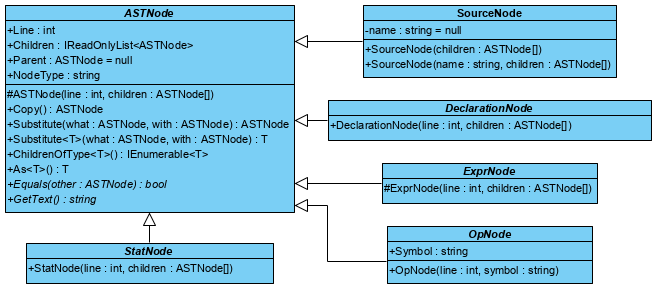
\includegraphics[scale=0.7]{images/uml/ASTNode.png}
\caption{Korisniči interfejs programa pružen kroz argumente komandne linije.}
\label{fig:UIImpl}
\end{figure}

\section{Testovi}
\label{sec:ImplementationTests}

Komponentu za kreiranje AST i komponentu za poređenje AST prate testovi jedinica koda. Testovi su organizovani u zasebnom projektu na sledeći način:
\begin{itemize}
    \item \texttt{LICC.Tests.AST} --- Testovi za adaptere i posetioce, kao i testovi funkcionalnosti metoda klase \texttt{ASTNode}.
    \item \texttt{LICC.Tests.Core} --- Testovi upoređivača.
\end{itemize}

Radni okvir koji se koristi za testiranje je \texttt{NUnit}\footnote{\url{https://nunit.org/}} koji pruža tzv. \emph{model ograničenja} (engl. \emph{constraint model}) i time omogućava pisanje čitljivog koda. Pisanje testova po modelu ograničenja se sastoji od korišćenja jednog metoda za pisanje svih testova koji kao argumente prima objekat koji se testira i složeni objekat koji predstavlja ograničenje koje objekat koji se testira treba da zadovoljava. Primer testa pisanog u ovom radnom okviru uz model ograničenja u kontekstu implementacije ovog rada se može videti na slici \ref{fig:ImplTestsUnit}.

\begin{figure}[h!]
\centering
\begin{lstlisting}
[Test]
public void ComplexDefinitionTest()
{
    FuncDefNode f = this.AssertFunctionSignature(@"
        float f(const unsigned int x, ...) {
            int z = 4;
            return 3.0;
        }", 
        2, "f", "float", isVariadic: true, 
        @params: ("unsigned int", "x")
    );
    Assert.That(f.IsVariadic);
    Assert.That(f.Definition.Children, Has.Exactly(2).Items);
}

protected FuncDefNode AssertFunctionSignature(
    string src, int line, string fname, 
    string returnType = "void", bool isVariadic = false, 
    AccessModifiers access = AccessModifiers.Unspecified,
    QualifierFlags qualifiers = QualifierFlags.None, 
    params (string Type, string Identifier)[] @params)
{
    FuncDefNode f = this.GenerateAST(src).As<FuncDefNode>();
    this.AssertChildrenParentProperties(f);
    this.AssertChildrenParentProperties(f.Definition);
    Assert.That(f, Is.Not.Null);
    Assert.That(f.Line, Is.EqualTo(line));
    Assert.That(f.Declarator, Is.Not.Null);
    Assert.That(f.Declarator.Parent, Is.EqualTo(f));
    Assert.That(f.Keywords.AccessModifiers, Is.EqualTo(access));
    Assert.That(f.Keywords.QualifierFlags, Is.EqualTo(qualifiers));
    Assert.That(f.Identifier, Is.EqualTo(fname));
    Assert.That(f.ReturnTypeName, Is.EqualTo(returnType));
    Assert.That(f.IsVariadic, Is.EqualTo(isVariadic));
    if (@params?.Any() ?? false) {
        Assert.That(f.Parameters, Is.Not.Null);
        Assert.That(f.Parameters, Has.Exactly(@params.Length).Items);
        Assert.That(f.ParametersNode, Is.Not.Null);
        Assert.That(
            f.Parameters.Select(
                p => (p.Specifiers.TypeName, p.Declarator.Identifier)
            ), 
            Is.EqualTo(@params)
        );
    }
    return f;
}
\end{lstlisting}
\caption{Primer jediničnog testa za proveru generisanog AST čvora za datu funkciju.}
\label{fig:ImplTestsUnit}
\end{figure}

Osim testova jedinica koda, prisutni su i testovi integracije svih komponenti. Kao što je opisano u prethodnim odeljcima, rezultat rada adaptera je AST, dok je rezultat data upoređivača za data dva stabla kolekcija problema. Ta dva odvojena procesa se onda mogu spojiti kako bi se testirala integracija te dve komponente --- dakle, od dva programa očekivati određenu kolekciju problema. Primer za \emph{swap} algoritam se može videti na slici \ref{fig:ImplTestsIntegration}.

\begin{figure}[h!]
\centering
\begin{lstlisting}
[Test]
public override void DifferenceTests()
{
    this.Compare(
        this.FromPseudoSource(@"
            algorithm Swap 
            begin
                declare integer x = vx
                declare integer y = vy
                procedure swap()
                begin
                    declare integer tmp = x
                    x = y  
                    y = tmp
                end
            end
        "),
        this.FromCSource(@"
            int x = vx, y = vy;
            void swap() {
                int tmp = x; y = tmp; x = y;
            }
        "),
        new MatchIssues()
            .AddError(
                new BlockEndValueMismatchError("x", 1, "vy", "vx")
            )
            .AddError(
                new BlockEndValueMismatchError("x", 3, "vy", "vx")
            )
    );
}

protected void Compare(ASTNode src, ASTNode dst, 
    MatchIssues? expectedIssues = null)
{
    expectedIssues ??= new MatchIssues();
    MatchIssues issues = new ASTNodeComparer(src, dst)
        .AttemptMatch();
    Assert.That(issues, Is.EquivallentTo(expectedIssues));
}
\end{lstlisting}
\caption{Primer kompletnog testa za algoritam \emph{swap}.}
\label{fig:ImplTestsIntegration}
\end{figure}


\chapter{Zaključak}
\label{chp:conclusion}

U tezi je opisan način posmatranja apstrakne sintakse programa kroz AST, opisan je proces kreiranja AST od proizvoljne gramatike programskog jezika i opšte-prihvaćen interfejs za obilazak istog. Opisan je model opšte AST apstrakcije sa ciljem dovođenja imperativnih i skript jezika na isti nivo apstrakcije. Ova apstrakcija je korišćena za određivanje semantičke ekvivalentnosti strukturno sličnih segmenata koda kroz naivni algoritam poređenja vrednosti na krajevima blokova.

Kao glavni doprinos teze, implementiran je računarski program za kreiranje opšteg AST od izvorne datoteke, serijalizaciju i prikaz istog. Mehanizam dobijanja opšteg AST omogućava jednostavno proširenje za već postojeće ali i za proizvoljne gramatike, kroz implementaciju adaptera za tu gramatiku koji služi kao posrednik između stabla parsiranja i opšteg AST. Dodatno, kao jedna primena opšte AST apstrakcije, implementiran je opisani algoritam za semantičko poređenje kroz proširiv model upoređivača tipova opštih AST čvorova. Priloženo je par primera upotrebe na segmentima koda programskih jezika C, Lua i pseudojezika (kao primera proizvoljnog programskog jezika, definisanog specifično za ovaj rad).

Naredni koraci u dizajniranju modela opšte apstrakcije bi bili usmereni na podršku za korisnički definisane tipove kroz čvorove za opis klasa, struktura i enumeracija. Takođe, klase se u skript jezicima često izbegavaju tako što se podaci smeste u mapu gde ključevi imitiraju atribute klase. Stoga bi bilo poželjno imati i interfejs za kreiranje mape objekta od datog klasnog čvora i obrnuto. Postoji i potreba za apstrahovanjem čestih struktura podataka kao što su skupovi, torke i redovi sa prioritetom. Na taj način, ako se u jednom programu koristi niz, a u drugom lista sa definisanim indeksnim pristupom, moguće je vršiti analizu uz potencijalno upozorenje o gubitku na efikasnosti.


% ------------------------------------------------------------------------------
% Literatura
% ------------------------------------------------------------------------------
\literatura

% ==============================================================================
% Završni deo teze i prilozi
\backmatter
% ==============================================================================

% ------------------------------------------------------------------------------
% Biografija kandidata
\begin{biografija}
  \textbf{Ivan Ž. Ristović} rođen je 17.01.1995. godine u Užicu. Osnovnu školu, kao i 
  prirodno-matematički smer Užičke gimnazije, završio je kao nosilac Vukove diplome. 
  Tokom navedenog perioda školovanja isticao se u oblastima matematike, informatike, 
  fizike, hemije i engleskog jezika, što potvrđuje veći broj nagrada na Državnim 
  takmičenjima.

  Smer Informatika na Matematičkom fakultetu Univerziteta u Beogradu upisuje 2014. 
  godine. Na navedenom smeru je diplomirao 2018. godine, posle tri godine studija 
  sa prosečnom ocenom 9,17. Master studije upisuje na istom fakultetu odmah nakon 
  diplomiranja.
  
  U avgustu 2018. biva izabran u zvanje „Saradnik u nastavi“ na Matematičkom 
  fakultetu paralelno sa master studijama. Drži vežbe iz kurseva "Računarske mreže",
  "Funkcionalno programiranje", "Programske paradigme" i "Objektno orijentisano 
  programiranje" na kasnijim godinama osnovnih studija.
  
  Oblasti interesovanja uključuju pre svega razvoj i verifikaciju softvera, mikroservise 
  i računarske mreže.
\end{biografija}
% ------------------------------------------------------------------------------

\end{document}
